\cleardoublepage
\chapter{Video Coding Transforms} \label{chap:trans}

%%%%%%%%%%%%%%%%%%%%%%%%%%%%%%%%%%%%%%%%%%%%%%%%%%%%%%%%%%%%%%%%%%%%%%%%%%%%%%
\section{{Introduction}}

As mentioned previously, the basic principle behind the compression of video, is the reduction of inter-pixel/inter-symbol correlation. The various integral blocks of a video compression system try to accomplish this objective through different strategies. The \emph{Intra-frame} and \emph{Inter-frame Prediction} exploit spatial and temporal correlation, respectively. Through the subtraction of the input by the output of one of these blocks, and the attainment of the \emph{residue}, the next compression stage is made in the \emph{Transform} block, which is the focus of this work.

The technique implemented by this process relies on the energy compaction in the frequency domain to reduce the correlation within a frame block, i.e. the input of the Transform block is evaluated on its main frequencies --- the \emph{transform coefficients} --- on a spatial domain, similarly to the process executed on a \emph{Fourier Transform}. Once each block is quantized on these coefficients, the compression is made with the removal of the least significant ones, on the \emph{Quantization} stage. The intent of the \emph{transform} is to split the image into a set of predefined coefficients, that get transmitted in place of the \emph{residue}.

The objective of this chapter is to give the reader a basic understanding of the theoretical basis behind said Transformations, as well as to introduce the most commonly used ones. 

%%%%%%%%%%%%%%%%%%%%%%%%%%%%%%%%%%%%%%%%%%%%%%%%%%%%%%%%%%%%%%%%%%%%%%%%%%%%%%
\section{Background}
%%%%%%%%%%%%%%%%%%%%%%%%%%%%%%%%%%%%%%%
\subsection{Basis vector/image interpretation}

A useful interpretation, and a good starting point to the study of this process, is to see it as the decomposition of the input as a set of basis vectors (1D transforms) or images/matrices (2D transforms). The transformation outputs , $T_i$, can be seen as the weights of each basis vector/image, $\vec{e_i}$, that summed return the input, $\vec{g}$, i.e.

\begin{equation}
    \vec{g} = \sum_{i=1}^{N} T_i \vec{e_i}
\end{equation}
which means that the coefficients are related to the amount of correlation between the input and each basis component, and can be obtained with the \emph{inner product} of the input and each basis vector.

\begin{equation} \label{eq:coef_vec}
    T_i = \vec{e_i}^T \vec{g}
\end{equation}

Since each input vector will have different correlation values between the various basis vectors, this operation accomplishes two main objectives:

\begin{itemize}
    \item De-correlation of the input values
    \item Signaling of the most important basis vectors.
\end{itemize}

Considering a 2D image, $g(x,y)$, and its corresponding transformed coefficients, $T(u,v)$, where $(x,y)$ are the pixel coordinates, and $(u,v)$ are the corresponding coordinates in the transform domain, we can obtain an analogous version of equation \ref{eq:coef_vec} as

\begin{equation} \label{eq:Tmatsum}
    T(u,v) = \sum_{x=0}^{M-1}\sum_{y=0}^{N-1}g(x,y)f(x,y,u,v)
\end{equation}

Similarly, we can re-obtain the original picture

\begin{equation} \label{eq:Gmatsum}
    g(x,y) = \sum_{u=0}^{M-1}\sum_{v=0}^{N-1}T(u,v)i(x,y,u,v)
\end{equation}
where $f(x,y,u,v)$ and $i(x,y,u,v)$ are the \emph{forward} and \emph{inverse transformation kernels}\label{par:kernel}. To better explain the concept of these, first it's needed to introduce the two following concepts.

%%%%%%%%%%%%%%%%%%%%%%%%%%%%%%%%%%%%%%%%%%%
% ATTENTION: "BETTER EXPLAIN ... FIRST IT'S NEEDED" gives the idea that there is going to be a later explanation
%%%%%%%%%%%%%%%%%%%%%%%%%%%%%%%%%%%%%%%%%%%

%%%%%%%%%%%%%%%%%%%
\subsubsection{Separability}

A useful characteristic of 2D Video Coding Transforms is its ability to be independently calculated between rows and columns. This means that given a 2D block as input, the transform coefficients can be calculated first with the \emph{horizontal transform}, and then with the \emph{vertical transform}, or vice-versa.

This aspect is applicable if the following conditions are applied

\begin{equation} \label{eq:fwf1f2}
    f(x,y,u,v)=f_1(x,u)f_2(y,v)
\end{equation}


\begin{equation} \label{eq:ini1i2}
    i(x,y,u,v)=i_1(x,u)i_2(y,v)
\end{equation}

This means that the equation \ref{eq:Tmatsum} is reconstructed as 2 independent and sequential operations

\begin{gather}
    T_{temp}(x,v) = \sum_{y=0}^{N-1}g(x,y)f_2(y,v) \\
    T(u,v) = \sum_{x=0}^{M-1}T_{temp}(x,v)f_1(x,u)
\end{gather}

On AV1, due to the various implemented transformation kernels, this aspect is severely explored, since the only way of implementing the combination of different 1D kernels, is to calculate them independently. This aspect is further explained with the following concept.

%%%%%%%%%%%%%%%%%%%
\subsubsection{Symmetry}

Taking equation \ref{eq:fwf1f2}, a transformation kernel is said to be symmetric if 

\begin{equation}
    f_1(y,v) = f_2(x,u)
\end{equation}

This characteristic is particularly useful because it makes the forward and inverse transformations expressible as matrix multiplications. Therefore, the equations \ref{eq:Tmatsum} and \ref{eq:Gmatsum} are represented, respectively, as

\begin{equation}
    T = F^TGF 
\end{equation}
\begin{equation}
    G = I^TTI
\end{equation}
where $F$ and $I$ are the forward and inverse transform matrices. This aspect is only possible for square matrix, i.e., input blocks with the same height and width.

This concept isn't exploited in AV1, since the use of different 1D transformation kernels, and rectangular block sizes ($M \neq N$) make the 2D transform asymmetric, and therefore, not executable as matrix multiplication. Consequently, the block transformation is made as 2 separate 1D operations, as shown previously.


\textsep

Looking now at equation \ref{eq:Gmatsum}, we can interpret the inverse transformation kernel as a set of basis images, dependent of the $(u,v)$ pair. By this, it is meant 

\begin{equation}
    g(x,y) = \sum_{u=0}^{M-1}\sum_{v=0}^{N-1}T(u,v)I_{u,v}
\end{equation}
where

\begin{equation}
    I_{u,v}=\begin{bmatrix}
                i(0,0,u,v) & i(0,1,u,v) & \dots & i(0,M-1,u,v) \\
                i(1,0,u,v) & i(1,1,u,v) & \dots & i(1,M-1,u,v) \\
                \vdots     & \vdots     & \dots & \vdots       \\
                i(N-1,0,u,v) & i(N-1,1,u,v) & \dots & i(N-1,M-1,u,v) \\
            \end{bmatrix}
\end{equation}

Therefore, the forward and inverse transformation process can be seen as the deconstruction of an input block, into a set of $M \cdot N$ basis images, dependent of the used transformation kernel. As expressed in equations \ref{eq:fwf1f2} and \ref{eq:ini1i2}, this analogy can be made on a 1D space \nocite{shiImageVideoCompression2008}.

%\todo[inline,color=red!40]{JPEG example?}

Given a general comprehension of the theoretical principles behind the \emph{Transform} block, now the most common transformation kernels are introduced, with focus on the AV1 video codec.

%%%%%%%%%%%%%%%%%%%%%%%%%%%%%%%%%%%%%%%%%%%%%%%%%%%%%%%%%%%%%%%%%%%%%%%%%%%%%%
\section{Transformation Kernels} \label{sec:kernels}

%%%%%%%%%%%%%%%%%%%%%%%%%%%%%%%%%%%%%%%
\subsection{Discrete Fourier Transform (DFT)}

Although it isn't implemented in video coding, it's widely used in digital signal processing, and many of the used transformation kernels are approximations of this function.

It has it's roots on the \emph{Fourier Transform}, whose forward and inverse transformations are expressed in equations \ref{eq:fourf} and \ref{eq:fouri}, respectively.

\begin{equation} \label{eq:fourf}
    T(u,v) = \int_{-\infty}^{\infty}\int_{-\infty}^{\infty}g(x,y)e^{-j2\pi(ux+vy)} dx \, dy
\end{equation}

\begin{equation} \label{eq:fouri}
    g(x,y) = \int_{-\infty}^{\infty}\int_{-\infty}^{\infty}T(u,v)e^{j2\pi(ux+vy)} du \, dv
\end{equation}

Once considered a finite number of points, the previous equations become

\begin{equation} \label{eq:dftf}
    T(u,v) = \frac{1}{MN}\sum_{x=0}^{M-1}\sum_{y=0}^{N-1}g(x,y)e^{-j2\pi \left(\frac{ux}{M}+\frac{vy}{N}\right)}
\end{equation}

\begin{equation} \label{eq:dfti}
    g(x,y) = \sum_{u=0}^{M-1}\sum_{v=0}^{N-1}T(u,v)e^{j2\pi \left(\frac{ux}{M}+\frac{vy}{N}\right)}
\end{equation}
which corresponds to replacing the kernels in equations \ref{eq:Tmatsum} and \ref{eq:Gmatsum} with

\begin{gather}
    f(x,y,u,v) = \frac{1}{MN} e^{-j2\pi \left(\frac{ux}{M}+\frac{vy}{N}\right)} \\
    i(x,y,u,v) = e^{j2\pi \left(\frac{ux}{M}+\frac{vy}{N}\right)}
\end{gather}

The position of the multiplication factor, $\frac{1}{MN}$, is irrelevant, and in some works is divided into two terms in the forward and inverse kernels, $\frac{1}{M}$ and $\frac{1}{N}$, or even $\frac{1}{\sqrt{MN}}$. \nocite{gonzalezDigitalImageProcessing2018}

Because of the use of complex numbers, this operation tends require a high computational effort, whence its disuse in video coding.

%%%%%%%%%%%%%%%%%%%%%%%%%%%%%%%%%%%%%%%
\subsection{Discrete Walsh-Hadamard Transform (WHT)}

This transformation replaces the sum of sines and cosines of the DFT, alternating of positive and negative $1$'s, depending on the binary representation of the inputs.

Considering the inputs of the transform to be represented with $m$ bits, where $m-1$ is the most significant bit ($b_{m-1}$), the forward and inverse kernels are represented as

\begin{equation}
    f(x,y,u,v) = i(x,y,u,v) = \frac{1}{\sqrt{MN}}(-1)^{\sum_{i=0}^{m-1}\lfloor b_i(x)p_i(u)+b_i(y)p_i(v)\rfloor}
\end{equation}
where

\begin{align*}
    &p_0(u)=b_{m-1}(u) \\
    &p_1(u)=b_{m-1}(u) +b_{m-2}(u) \\
    \,&\vdots \addtocounter{equation}{1}\tag{\theequation} \\
    &p_{m-1}(u)=b_1(u)+b_0(u) 
\end{align*}

%%%%%%%%%%%%%%%%%%%%%%%%%%%%%%%%%%%%%%%
\subsection{Discrete Cosine Transform (DCT)}

The most commonly used transform, the \emph{DCT}, was published by Ahmed et al. in 1974 \cite{ahmedDiscreteCosineTransform1974}. Since then, it has been adopted in a wide range of applications, being the only transform used in the first generations of video codecs, as well as in \emph{still image compression}, being the basis of the \emph{\gls{JPEG}} standard.

It is frequently compared to the \emph{DFT}, due to the similarity of their operation. However, as the name implies, the \emph{DCT} relies on the cosine function to create its basis images, which is a \emph{periodic} and \emph{symmetrically even} function. Therefore, as mentioned by \cite[A. V. Oppenheim]{oppenheimDiscretetimeSignalProcessing1998}, \emph{"Just as the DFT involves an implicit assumption of periodicity, the DCT involves implicit assumptions of both periodicity and even symmetry"}.  This is easily observable once considered the equivalent process of both algorithms. Taking an $N$-point sequence, $g(n)$, the calculation of the \emph{DFT} and \emph{DCT} of such sequence is equivalent to the processes presented at table \ref{tab:DFTDCT}.

\begin{table}[!htpb]
    \centering
    \begin{tabular}{cllll@{}} \toprule
        \textbf{Step} &      \multicolumn{2}{c}{\textbf{\emph{DFT}}} &      \multicolumn{2}{c}{\textbf{\emph{DCT}}} \\ \toprule
        1 &         \multicolumn{2}{p{0.35\textwidth}}{Repeat $g(n)$ every N points, giving origin to $\widetilde{g}_N(n)$} &         \multicolumn{2}{p{0.35\textwidth}}{Concatenate $g(n)$ with a flipped version of itself, creating a $2N$ sequence, $g_{2N}(n)$, and repeat it, giving origin to $\widetilde{g}_{2N}(n)$}\\ 
        2 &         \multicolumn{2}{p{0.35\textwidth}}{Calculate the \emph{Fourier} expansion of $\widetilde{g}_N$} &         \multicolumn{2}{p{0.35\textwidth}}{Calculate the \emph{Fourier} expansion of $\widetilde{g}_{2N}$}\\ 
        3 &         \multicolumn{2}{p{0.35\textwidth}}{Keep the first $N$ coefficients\, and set all others to $0$} &         \multicolumn{2}{p{0.35\textwidth}}{Keep the first $N$ coefficients, and set all others to $0$}\\ 
        \bottomrule
    \end{tabular}
    \caption{Similarity between the processes of the        \emph{DFT} and the \emph{DCT}}
    \label{tab:DFTDCT}
\end{table}

The main reason behind the heavy adoption of the \emph{DCT} is its great energy compaction on the lower frequencies, where most of the energy in a picture is packed. If the output of the first step of table \ref{tab:DFTDCT} is observed, this aspect is more easily understood. In figure \ref{fig:2NSeq}, a 4 point sequence, corresponding to the filled points, gets replicated throughout the discrete time axis, according to the corresponding transform.

Due to the back-to-head repetition seen in figure \ref{subfig:dft}, there is a disruption every $N$ points, which gives origin to high frequency components in the \emph{Fourier} transform. Therefore, the more continuous behavior obtained with the back-to-back repetition of the \emph{DCT} gives origin to more significant low frequency coefficients. However, there are many ways of creating a periodic and symmetric sequence from a finite number of points. This factor has led to the implementation of different versions of the \emph{DCT}, which differ in minor details between themselves. These differences are consequence of the way the symmetry is obtained, which can be observed in figures \ref{subfig:dct1} to \ref{subfig:dct4}. The represented implementations are referred to as \emph{DCT-I} to \emph{DCT-IV}, but other possibilities exist. Their definition depends on the overlapping of points when repeating each sequence.

\begin{figure}[!htpb]
    \centering 
        \begin{subfigure}[c]{\textwidth}
            \centering
            \begin{tikzpicture}[scale=0.5]
    \draw[thick,->] (-1,0) -- (13,0) node[anchor=north west] {$n$};
    \foreach \x in {1,...,12}
        \draw (\x cm,1pt) -- (\x cm,-1pt) node[anchor=north] {};%{$\x$};
    \draw[thick,->] (0,-1) -- (0,5) node[anchor=south east] {};
    
    \foreach \x in {0,...,3} {
        \filldraw[fill=black, black] (\x cm,4-\x) circle (0.1cm);
        \draw [black] (\x,4-\x) -- (\x,0);
    }

    \foreach \x in {4,...,7} {
        \draw[draw=black] (\x cm,4-\x+4) circle (0.1cm);
        \draw (\x,4-\x+4) -- (\x,0);
    }

    \foreach \x in {8,...,11} {
        \draw[draw=black] (\x cm,4-\x+8) circle (0.1cm);
        \draw (\x,4-\x+8) -- (\x,0);
    }

    \draw[draw=black] (12 cm,4) circle (0.1cm);
    \draw (12,4) -- (12,0);

\end{tikzpicture}
            \caption{\emph{DFT}}
            \label{subfig:dft}
        \end{subfigure}
        \begin{subfigure}[c]{0.45\textwidth}
            \centering
            \begin{tikzpicture}[scale=0.45]
    \draw[thick,->] (-1,0) -- (13,0) node[anchor=north west] {$n$};
    \foreach \x in {1,...,12}
        \draw (\x cm,1pt) -- (\x cm,-1pt) node[anchor=north] {$\x$};
    \draw[thick,->] (0,-1) -- (0,5) node[anchor=south east] {};
    
    \foreach \x in {0,...,3} {
        \filldraw[fill=black, draw=black] (\x cm,4-\x) circle (0.1cm);
        \draw (\x,4-\x) -- (\x,0);
    }

    \foreach \x in {4,...,6} {
        \draw[draw=black] (\x cm,\x-2) circle (0.1cm);
        \draw (\x,\x-2) -- (\x,0);
    }

    \foreach \x in {7,...,9} {
        \draw[draw=black] (\x cm,4-\x+6) circle (0.1cm);
        \draw (\x, 4-\x+6) -- (\x,0);
    }

    \foreach \x in {10,...,12} {
        \draw[draw=black] (\x cm,\x-8) circle (0.1cm);
        \draw (\x, \x-8) -- (\x,0);
    }
\end{tikzpicture}
            \caption{\emph{DCT-I}}
            \label{subfig:dct1}
        \end{subfigure}
        \begin{subfigure}[c]{0.45\textwidth}
            \centering
            \begin{tikzpicture}[scale=0.45]
    \draw[thick,->] (-1,0) -- (13,0) node[anchor=north west] {$n$};
    \foreach \x in {1,...,12}
        \draw (\x cm,1pt) -- (\x cm,-1pt) node[anchor=north] {};%{$\x$};
    \draw[thick,->] (0,-1) -- (0,5) node[anchor=south east] {};
    
    \foreach \x in {0,...,3} {
        \filldraw[fill=black, draw=black] (\x cm,4-\x) circle (0.1cm);
        \draw (\x,4-\x) -- (\x,0);
    }

    \foreach \x in {4,...,7} {
        \draw[draw=black] (\x cm,\x-3) circle (0.1cm);
        \draw (\x,\x-3) -- (\x,0);
    }

    \foreach \x in {8,...,11} {
        \draw[draw=black] (\x cm,4-\x+8) circle (0.1cm);
        \draw (\x, 4-\x+8) -- (\x,0);
    }

    \draw[draw=black] (12 cm,1) circle (0.1cm);
    \draw (12, 1) -- (12,0);

\end{tikzpicture}
            \caption{\emph{DCT-II}}
            \label{subfig:dct2}
        \end{subfigure}
        \begin{subfigure}[c]{0.45\textwidth}
            \centering
            \begin{tikzpicture}[scale=0.45]
    \draw[thick,->] (-1,0) -- (13,0) node[anchor=north west] {$n$};
    \foreach \x in {1,...,4}
        \draw (\x cm,1pt) -- (\x cm,-1pt) node[anchor=north] {$\x$};
    \foreach \x in {5,...,12}
        \draw (\x cm,1pt) -- (\x cm,-1pt) node[anchor=south] {$\x$};
    \draw[thick,->] (0,-1) -- (0,5) node[anchor=south east] {};
    
    \foreach \x in {0,...,3} {
        \filldraw[fill=black, draw=black] (\x cm,4-\x) circle (0.1cm);
        \draw (\x,4-\x) -- (\x,0);
    }
    \foreach \x in {4,...,8} {
        \draw[draw=black] (\x cm,4-\x) circle (0.1cm);
        \draw (\x,4-\x) -- (\x,0);
    }

    \foreach \x in {9,...,12} {
        \draw[draw=black] (\x cm,\x-12) circle (0.1cm);
        \draw (\x,\x-12) -- (\x,0);
    }

\end{tikzpicture}
            \caption{\emph{DCT-III}}
            \label{subfig:dct3}
        \end{subfigure}
        \begin{subfigure}[c]{0.45\textwidth}
            \centering
            \begin{tikzpicture}[scale=0.45]
    \draw[thick,->] (-1,0) -- (13,0) node[anchor=north west] {$n$};
    \foreach \x in {1,...,3}
        \draw (\x cm,1pt) -- (\x cm,-1pt) node[anchor=north] {};%{$\x$};
    \foreach \x in {4,...,11}
        \draw (\x cm,1pt) -- (\x cm,-1pt) node[anchor=south] {};%{$\x$};
    \draw (12 cm,1pt) -- (12 cm,-1pt) node[anchor=north] {};%{12};
    \draw[thick,->] (0,-1) -- (0,5) node[anchor=south east] {};
    
    \foreach \x in {0,...,3} {
        \filldraw[fill=black, draw=black] (\x cm,4-\x) circle (0.1cm);
        \draw (\x,4-\x) -- (\x,0);
    }

    \foreach \x in {4,...,7} {
        \draw[draw=black] (\x cm,-\x+3) circle (0.1cm);
        \draw (\x,-\x+3) -- (\x,0);
    }

    \foreach \x in {8,...,11} {
        \draw[draw=black] (\x cm,-12+\x) circle (0.1cm);
        \draw (\x, -12+\x) -- (\x,0);
    }

    \draw[draw=black] (12 cm,1) circle (0.1cm);
    \draw (12, 1) -- (12,0);

\end{tikzpicture}
            \caption{\emph{DCT-IV}}
            \label{subfig:dct4}
        \end{subfigure}
        \caption{Sequences generated in the first step of table \ref{tab:DFTDCT}for the DFT and different DCTs. Filled dots correspond to the original sequence.}
    \label{fig:2NSeq}
\end{figure}

%Of the different implementations, \emph{DCT-1} and \emph{DCT-2} are the most commonly used, being the \textcolor{red}{focus of this work}. 

Since the \emph{DCT} in \emph{AV1} is implemented in one dimension, the description of the following kernels is also made in 1D. Therefore, the dimension of the transform, $L$, is referring either to the blocks' width or height, depending if the operation is made to the rows or columns, respectively ($M$ or $N$, previously).

%%%%%%%%%%%%%%%%%%%
\paragraph{DCT-I}

The sequence created with first version of the DCT has overlapping points at $n = k(L-1) ,\ k = 0,1,2,...$, making the overall period of the final sequence $2L-2$.

\begin{equation}
    f(x,u) = \frac{2}{L-1}\alpha(x)\cos\left(\frac{\pi xu}{L-1}\right)
\end{equation}
where

\begin{equation}
    \alpha(x)= \begin{cases}
                    \frac{1}{2}, & x=0 \lor x = N-1 \\
                    1, & 1 \leq x \leq N-2
                \end{cases}
\end{equation}

The inverse transform becomes
\begin{equation}
    i(x,u) = \alpha(u)\cos\left(\frac{xu\pi}{L-1}\right)
\end{equation}

%%%%%%%%%%%%%%%%%%%
\paragraph{DCT-II}

Usually referred to as "the \emph{DCT}", it is by far the most implemented version, being the only one mentioned in many of the studied works.

As seen in figure \ref{subfig:dct2}, this version has no overlap on the created sequence, making the period $2L$, and the points of symmetry $kL - \frac{1}{2}$.

\begin{gather}
    f(x,u) = i(x,u) = \beta(u)\cos\left(\frac{(2x+1)u\pi }{2L}\right) \\
    \beta(u)= \begin{cases}
                    \sqrt{\frac{1}{L}}, & u=0 \\
                    \sqrt{\frac{2}{L}}, & 1 \leq u \leq N-1
                \end{cases}
\end{gather}

%%%%%%%%%%%%%%%%%%%
\paragraph{DCT-III}
Named the \emph{inverse} of DCT-II, due to the switch of the transform and pixel coordinates.

\begin{gather}
    f(x,u) = i(x,u) = \beta(u)\cos\left(\frac{(2u+1)x\pi }{2L}\right) \\
    \beta(u)= \begin{cases}
                    \sqrt{\frac{1}{L}}, & u=0 \\
                    \sqrt{\frac{2}{L}}, & 1 \leq u \leq N-1
                \end{cases}
\end{gather}

%%%%%%%%%%%%%%%%%%%
\paragraph{DCT-IV}

Is the basis of the \emph{Modified Discrete Cosine Function (MDCT)}, where the input blocks overlap.

\nocite{DiscreteCosineTransform}

\begin{equation}
    f(x,u) = i(x,u) = \sqrt{\frac{2}{L}}\cos\left(\frac{(2u+1)(2x+1)\pi }{4L}\right)
\end{equation}

%%%%%%%%%%%%%%%%%%%%%%%%%%%%%%%%%%%%%%%
\subsection{Discrete Sine Transform (DST)}

\nocite{prattDigitalImageProcessing2001}

Similarly to the DCT, there is also the possibility to represent a finite sequence as a sum of discrete \emph{sine} functions, giving origin to the \emph{DST}. Contrarily to the former presented transform, this variant uses sinusoidal functions to generate its basis images, which gives origin to \emph{odd symmetric} sequences.

In the same way as its \emph{even} counterpart, there are various different ways off accomplishing such symmetry, which also gives origin to eight different variations of this Transform. However, due to its misuse over the DCT, only the \emph{DST-II} is presented.

\begin{equation}
    f(x,u) = i(x,u) = \sqrt{\frac{2}{L+1}}\sin\left(\frac{(j+1)(u+1)\pi}{L+1}\right)
\end{equation}

Equivalently to what happens with the DFT, the odd symmetry of this function gives origin to discontinuities, which are undesirable when coding video blocks, since they lead to less significant low frequency coefficients, and therefore higher quantization errors.

%%%%%%%%%%%%%%%%%%%%%%%%%%%%%%%%%%%%%%%
\subsection{Asymmetric Discrete Sine Transform (ADST)}

\nocite{hanButterflyStructuredDesign2013}
\nocite{bingNextgenerationVideoCoding2015}

The symmetric behavior of previous transforms lead to better performance on evenly spread residue blocks, i.e. when the pixel values post-subtraction (and before transformation) have roughly the same value across the whole block.

However, due to the directional spatial prediction, the residue on one boundary of the block may be different from the other boundaries, since the chosen direction for prediction may diverge from the original block, across the prediction block. This leads to worse energy compression.

In order to combat this aspect, VP9 introduced a new transform called \emph{Asymmetric Discrete Sine Transform (ADST)}, which corresponds to an alternative implementation of the DST with the addition of frequency and phase shifts.

This enhancement provides the developer with a high degree of liberty, since the basis images can be adapted with the variation of the shifts. On AV1, there is only one ADST implementation per block size. However this transformation can be done in two directions, i. e., the input vector can be transformed front-to-back and vice-versa. \emph{AOMedia} named these transforms \emph{ADST} and \emph{Flip-ADST}, according to the direction of the input vector.

%\todo[inline,color=red!40]{AV1 ADST formula}

%%%%%%%%%%%%%%%%%%%%%%%%%%%%%%%%%%%%%%%%%%%%%%%%%%%%%%%%%%%%%%%%%%%%%%%%%%%%%%
\section{Libaom's Integer Transformations}
\nocite{soo-changpeiIntegerTransformsAnalogous2000}

In battery driven applications, computing power plays an important role. Consequently, any approach that leads to lower computational costs, without compromising the image quality, tends to get incorporated into a video codec.

When considering the transformation stage, a widely used approach is the use of \emph{integer transforms}. The objective of such operations is to maintain the features of floating point transforms, but severely reducing the complexity, decreasing the used operations to arithmetic additions and integer multiplications. In many implementations, the latter are implemented with bitwise shifts and additions.

From the transforms presented throughout section \ref{sec:kernels}, there have been several methods of developing integer counterparts. Most of the fast implementations are based in either \emph{Fast Fourier Transform} algorithms or in the \emph{Walsh-Hadamard Transform} \cite{wolterParallelArchitecturesDiscrete1992,yonghongzengIntegerDCTsFast2001}. Since the objective of this work was to develop a \emph{Transform Co-processor} for \emph{libaom}, the focus of this section resolves around these kernels. 

%%%%%%%%%%%%%%%%%%%%%%%%%%%%%%%%%%%%%%%
\subsection{Functioning and Implementation}

The first analysis of this section was made through the study of the transformation stage of the reference software. Its main workflow is represented in figure \ref{fig:libtrans}.

\begin{figure}[!htbp]
    \centering
    \begin{tikzpicture}[%
    >=triangle 60,              % Nice arrows; your taste may be different
    start chain=going below,    % General flow is top-to-bottom
    node distance=6mm and 40mm, % Global setup of box spacing
    every join/.style={norm},   % Default linetype for connecting boxes
    ]

\tikzset{
  base/.style={draw, on chain, on grid, align=center, minimum height=4ex},
  proc/.style={base, rectangle, text width=8em},
  test/.style={base, diamond, aspect=2, text width=6em},
  inout/.style={base,draw,trapezium,trapezium left angle=70,trapezium right angle=-70},
  term/.style={proc, rounded corners},
  % coord node style is used for placing corners of connecting lines
  coord/.style={coordinate, on chain, on grid, node distance=6mm and 40mm},
  % nmark node style is used for coordinate debugging marks
  nmark/.style={draw, cyan, circle, font={\sffamily\bfseries}},
  % -------------------------------------------------
  % Connector line styles for different parts of the diagram
  norm/.style={->, draw},
  free/.style={->, draw, green3},
  cong/.style={->, draw, red3},
  it/.style={font={\itshape}}
}    
    
  \begin{scope}

    \node[inout, it] (start) {Input Block};

    \node[proc, below=1.5cm of start] (get_col) {Get Column \texttt{i\_c}};
      \path (start.south) to node [near end, xshift=2em, text=blue!80!black] {\texttt{i\_c=0}} (get_col);
        \draw [->] (start.south) -- (get_col);
    
    \node[test, join] (ud_flip) {\texttt{ud\_flip}};      

    \node[proc] (T1) {$T$};
      \path (ud_flip.south) to node [near start, xshift=1em, text=red!80!black] {\texttt{0}} (T1);
          \draw [->] (ud_flip.south) -- (T1);
    
    \node[test, join] (lr_flip) {\texttt{lr\_flip}};   

    \node[proc] (store1) {Store coefficients};
      \path (lr_flip.south) to node [near start, xshift=1em, text=red!80!black] {\texttt{0}} (store1);
            \draw [->] (lr_flip.south) -- (store1);

    \node[test, join, text width=7em] (i_col) {\texttt{i\_c == (size\_col - 1)}};

    \node[proc,below=2.7cm of i_col] (get_row) {Get Row \texttt{i\_r}};
      \path (i_col.south) to node [near end, xshift=2em, yshift=-0.2em, text=blue!80!black] {\texttt{i\_r=0}} (get_row);
      \path (i_col.south) to node [near start, xshift=-1.5em, yshift=0.2cm, text=red!80!black] {\texttt{true}} (get_row);
        \draw [->] (i_col.south) -- (get_row);

    \node[proc, join] (T2) {$T$};

    \node[proc, join] (store2) {Store coefficients};

    \node[test, join, text width=7em] (i_row) {\texttt{i\_r == (size\_row - 1)}};

    \node[term,line width=0.8mm] (end) {End};      
      \path (i_row.south) to node [near start, xshift=-1.5em, text=red!80!black] {\texttt{true}} (end);
        \draw [->] (i_row.south) -- (end);

      \node[proc, right=of ud_flip] (flip_in) {Flip Input Vertically};
      \path (ud_flip.east) to node [near start, yshift=1em, text=red!80!black] {\texttt{1}} (flip_in);
          \draw [->] (ud_flip.east) -- (flip_in); 

      \node[coord, right=of T1] (T1_right) {};
      \path (flip_in.south) to node {} (T1_right);
        \draw [->] (flip_in.south) -- (T1_right) |- (T1);

      \node[proc, right=of lr_flip] (flip_in2) {Flip Coefficients Horizontally};
      \path (lr_flip.east) to node [near start, yshift=1em, text=red!80!black] {\texttt{1}} (flip_in2);
          \draw [->] (lr_flip.east) -- (flip_in2); 

      \node[coord, right=of store1] (store1_right) {};
      \path (flip_in2.south) to node {} (store1_right);
        \draw [->] (flip_in2.south) -- (store1_right) |- (store1);

      \node[coord, left=of get_col] (get_col_left) {};
      \path (get_col_left) to node [yshift=0.5em, text=blue!80!black] {\texttt{i\_c+=1}} (get_col);
      \node[coord, left=of i_col] (i_col_left) {};
      \path (i_col.west) to node [yshift=-1em, text=red!80!black] {\texttt{false}} (i_col_left);
        \draw [->] (i_col.west) -- (i_col_left) |- (get_col_left) |- (get_col);

      \node[coord, left=of get_row] (get_row_left) {};
      \path (get_row_left) to node [yshift=0.5em, text=blue!80!black] {\texttt{i\_r+=1}} (get_row);
      \node[coord, left=of i_row] (i_row_left) {};
      \path (i_row.west) to node [yshift=-1em, text=red!80!black] {\texttt{false}} (i_row_left);
        \draw [->] (i_row.west) -- (i_row_left) |- (get_row_left) |- (get_row);
  \end{scope}        
  
  \begin{pgfonlayer}{background}
    % Left-top corner of the background rectangle
    \path (get_col_left.west |- get_col_left.north)+(-1.5cm,0.8cm) node (a11) {};
    % Right-bottom corner of the background rectanle
    \path (flip_in.east |- i_col.south)+(+1cm,-0.5cm) node (a21) {};
    % Draw the background
    \path[fill=black!10,rounded corners, draw=black!50, dashed]
      (a11) rectangle (a21);
    \path (a11 |- a21) node (a31) {};
    \path (a11) -- (a31) node[midway, rotate=90, yshift=-0.5cm] (mid_right) {\textbf{Column Transform}};

    \path (get_row_left.west |- get_row_left.north)+(-1.5cm,0.8cm) node (a12) {};
    \path (flip_in.east |- i_row.south)+(+1cm,-0.3cm) node (a22) {};
    \path[fill=black!10,rounded corners, draw=black!50, dashed]
      (a12) rectangle (a22);
    \path (a12 |- a22) node (a32) {};
    \path (a12) -- (a32) node[midway, rotate=90, yshift=-0.5cm] (mid_right) {\textbf{Row Transform}};

  \end{pgfonlayer}
\end{tikzpicture}
    \caption{Flowchart of the Transform Stage on \emph{libaom}}
    \label{fig:libtrans}
\end{figure}

This stage is controlled by a configuration set, which is chosen according to the desired encoding objectives. These parameters control the transformation block width and height (\texttt{size\_col} and \texttt{size\_row} \footnote{Each number does not correspond to the number of elements in columns and rows, but rather to the number of rows and columns.}, respectively), the transformation kernels to use in the rows and columns, the precision to use in the sine and/or cosine coefficient approximations, as well as other parameters for overflow control. Associated to the transformation kernel chosen, the variables \texttt{ud\_flip} and \texttt{lr\_flip} are also set. The first one is set to \emph{\texttt{1}} if the block's columns are to be transformed with the \emph{Flip-ADST} kernel. If such choice is applied to the rows, the second variable is, likewise, set to \emph{\texttt{1}}. These variables control if the input rows are flipped vertically, and/or if the coefficients resulting from the column transformation are flipped horizontally \footnote{Here, the notation of \emph{horizontally} or \emph{vertically} is set considering a matrix input block. In the 1D transform implemented in \emph{libaom}, this just means that what would be the last coefficient is now the first, and so on.}.

The choosing of these parameters will not be addressed in this work, since \emph{AV1} allows for a great deal of maneuverability to the designer, as to adjust each encoder/decoder pair to the desired application. In this regard, \emph{libaom} allows for a high number of configuration options, that dramatically change the parameters chosen in the transformation stage, as well as in the rest of the system.

Throughout the represented process, many of the operations are done with sequential, iterative processes, e.g., the input vector selection or the flipping operations. Such operations would greatly benefit of a hardware implementation, since they are easily parallelizable, as the objectives of \emph{AV1} suggested. However, on this work, the focus relies of the \emph{T} block, i.e., the transformation itself.

Independently of the transformation kernel, the operation is done sequently, in various stages. In each of these, the corresponding intermediary coefficients get calculated as function of two of the previous calculated coefficients. These, in most of the stages, are multiplied by a specific integer approximation of cosine/sine value. Such approximations, as mentioned previously, depend on the number of bits on which they are represented. 

The arrays on which the calculated cosine and sine values are stored, \texttt{cospi} and \texttt{sinpi}, respectively, are bi-dimensional. The first dimension, $\texttt{N}$,  has 7 positions, where the first corresponds to 10 bit approximations, and the last to 16 bit. The second dimension, $\texttt{k}$, has 64 positions for \texttt{cospi} and 5 for \texttt{sinpi}, representing the first quadrant of the trigonometric circle. Each position is calculated according to equations \ref{eq:cos} and \ref{eq:sin}, where $k$ represents the position in the array, and $N$ corresponds to the number of bits. Therefore, \verb|cospi[N][0]| corresponds to $\cos(0)$, \verb|cospi[N][63]| is $\cos(63\pi/128)$, and the following positions can also be associated to a certain angle.

\begin{equation} \label{eq:cos}
    \texttt{cospi[N][k]} = \nint*{2^{N}\cos\left(\frac{k\pi}{128}\right)}
\end{equation}

\begin{equation} \label{eq:sin}
    \texttt{sinpi[N][k]} = 2^{N}\nint*{\frac{2}{3}\sqrt{2}\sin\left(\frac{k\pi}{9}\right)}
\end{equation}

The \texttt{sinpi} array is only used in the shortest length of the \emph{ADST}, which is the reason it only has five positions. All other versions of this kernel use \texttt{cospi} to get the desired value.

Most of the temporary coefficients inside each stage are calculated with the function \verb|half_btf|, which performs the operation represented in equation \ref{eq:half_btf}. This function takes the two previously calculated coefficients, two values from the previously introduced arrays, as well as the number of bits used to represent these, and maps the result from the multiplications and sum of the first inputs to the desired number of bits.

\begin{equation} \label{eq:half_btf}
    \texttt{half\_btf(w0, in0, w1, in1, bits)} \quad \widehat{=} \quad \nfloor*{\frac{w_0in_0 + w_1in_1 + 2^{bits -1}}{2^{bits}}}
\end{equation}

Although the code implementation is sequential, the \emph{8 length} transformation kernels are represented in figures \ref{fig:intDCT} and \ref{fig:intADST} as parallel block diagrams, with the diverse stages in series. While \emph{AV1} accepts \emph{transform block} sizes varying between 4 and 64, the method of transformation is similar between the different sizes.

Both pictures start with the input vector components, i.e., \texttt{x0} to \texttt{x7}. The following sum's represent the addition of the two pointing values, in case the that the arrow guiding these doesn't present any further coefficient. If such is verified, the operation to be realized is the one presented in equation \ref{eq:half_btf}. The value near each arrow is referred to the equivalent \texttt{cospi} position, that multiplies by the result coming from the arrow's origin. Figure \ref{fig:aid} presents a visual aid for the following figures.

The identity transforms, \emph{IDTX}, are the simplest of the ones implemented in \emph{libaom}, since they consist of a scale factor, which varies throughout the transform sizes.

On the 4 and 16 length transforms, the scaling factor includes a 12-bit integer approximation of the square root of 2, which is calculated through
\begin{equation}
    N_{\sqrt{2}}=\nint*{2^{12}\sqrt{2}}=5793
\end{equation}
Being so, the input also suffers an additional mapping, similar to the operation in \ref{eq:half_btf}. These operations are demonstrated in figure \ref{fig:intIDEN}.

\begin{figure}[!htbp]
    \centering
    \begin{tikzpicture}[%
    >={Triangle[length=6pt,angle'=28]},
    start chain=going below,    % General flow is left-to-right
    node distance=2mm and 20mm, % Global setup of box spacing
    every join/.style={norm},   % Default linetype for connecting boxes
    ]

\tikzset{
  base/.style={draw, on chain, on grid, align=center, minimum height=3.5ex},
  proc/.style={base, rectangle, text width=8em},
  inout/.style={base,trapezium,trapezium left angle=70,trapezium right angle=-70, fill=black!12},
  term/.style={proc, rounded corners},
  sum/.style={base, circle, inner sep=0pt, radius=0.4cm, fill=black!8},
  % coord node style is used for placing corners of connecting lines
  coord/.style={coordinate, on chain, on grid, node distance=6mm and 40mm},
  % nmark node style is used for coordinate debugging marks% -------------------------------------------------
  % Connector line styles for different parts of the diagram
  norm/.style={ar, draw},
  free/.style={ar, draw, green3},
  cong/.style={ar, draw, red3},
  it/.style={font={\small\itshape}},
  ar/.style={->, line width=0.4mm},
  nar/.style={ar, red!75!black},
  pathcos/.style={font=\small, sloped}
}

\begin{scope}
    \node [inout] (a1) {$A$};
    \node [inout] (b1) {$B$};

    \node [inout, below=2cm of a1] (a2) {$A$};
    \node [inout] (b2) {$B$};

    \node [inout, below=2cm of a2] (a3) {$A$};
    \node [inout] (b3) {$B$};

    \path (a1) -- (b1) node [midway] (s1t) {};
    \path (a2) -- (b2) node [midway] (s2t) {};
    \path (a3) -- (b3) node [midway] (s3t) {};

    \node [sum, right=of s1t] (s1) {\textbf{+}};
    \node [sum, right=of s2t] (s2) {\textbf{+}};
    \node [sum, right=of s3t] (s3) {\textbf{+}};

        \draw [ar] (a1.east) -- (s1);
        \draw [ar] (b1.east) -- (s1);

        \draw [ar] (a2.east) -- (s2);
        \draw [nar] (b2.east) -- (s2);

        \path (a3.east) to node [pathcos, above, near start] {$\alpha$} (s3.west);
            \draw [ar] (a3.east) -- (s3);
        \path (b3.east) to node [pathcos, color=red!75!black, below, near start] {$\beta$} (s3.west);
            \draw [nar] (b3.east) -- (s3);

    \node [inout, right=of s1] (c1) {$C$};        
    \node [inout, right=of s2] (c2) {$C$};
    \node [inout, right=of s3] (c3) {$C$};

        \draw [ar] (s1) -- (c1);
        \draw [ar] (s2) -- (c2);
        \draw [ar] (s3) -- (c3);

    \node [right=3.2cm of c1] (eq1) {$C = A + B$};
    \node [right=3.2cm of c2] (eq2) {$C = A - B$};
    \node [right=1cm of c3] (eq3) {$C = \,$\texttt{half\_btf(}$A, cospi_\alpha, B, -cospi_\beta, bits$\texttt{)}};
\end{scope}    

\begin{pgfonlayer}{background}
    \path (a1.west |- a1.north)+(-5mm,2mm) node (a11) {};
    \path (eq3.east |- b1.south)+(5mm,-2mm) node (a21) {};
    \path[fill=black!2,rounded corners, draw=black!50, dashed]
      (a11) rectangle (a21);

    \path (a2.west |- a2.north)+(-5mm,2mm) node (a11) {};
    \path (eq3.east |- b2.south)+(5mm,-2mm) node (a21) {};
    \path[fill=black!2,rounded corners, draw=black!50, dashed]
        (a11) rectangle (a21);

    \path (a3.west |- a3.north)+(-5mm,2mm) node (a11) {};
    \path (eq3.east |- b3.south)+(5mm,-2mm) node (a21) {};
    \path[fill=black!2,rounded corners, draw=black!50, dashed]
        (a11) rectangle (a21);
\end{pgfonlayer}
\end{tikzpicture}
    \caption{Graphical aid for figures \ref{fig:intDCT} and \ref{fig:intADST}}
    \label{fig:aid}
\end{figure}

\begin{figure}[!htbp]
    \centering
    \begin{tikzpicture}[%
    >={Triangle[length=6pt,angle'=28]},
    start chain=going below,    % General flow is left-to-right
    node distance=2mm and 28.8mm, % Global setup of box spacing
    every join/.style={norm},   % Default linetype for connecting boxes
    ]

\tikzset{
  base/.style={draw, on chain, on grid, align=center, minimum height=3.5ex},
  proc/.style={base, rectangle, text width=8em},
  inout/.style={base,trapezium,trapezium left angle=70,trapezium right angle=-70},
  term/.style={proc, rounded corners},
  sum/.style={base, circle, inner sep=0pt, radius=0.4cm},
  % coord node style is used for placing corners of connecting lines
  coord/.style={coordinate, on chain, on grid, node distance=6mm and 40mm},
  % nmark node style is used for coordinate debugging marks% -------------------------------------------------
  % Connector line styles for different parts of the diagram
  norm/.style={aar, draw},
  free/.style={aar, draw, green3},
  cong/.style={aar, draw, red3},
  it/.style={font={\small\itshape}},
  ar/.style={aar},
  nar/.style={aar, red!75!black},
  aar/.style={->},
  pathcos/.style={font=\small, sloped}
}    

\begin{scope}
    %% Stage 1
    \foreach \x in {0,...,7}
        \node [inout] (x\x) {\texttt{x\x}};

    \node [sum, right=of x0] (s10) {\textbf{+}};
    \foreach \x in {1,...,7}
        \node [sum] (s1\x) {\textbf{+}};
    
    \draw [aar] (x0.east) -- (s10);
    \draw [aar] (x0.east) -- (s17);         
    \draw [aar] (x1.east) -- (s11);
    \draw [aar] (x1.east) -- (s16);
    \draw [aar] (x2.east) -- (s12);
    \draw [aar] (x2.east) -- (s15);         
    \draw [aar] (x3.east) -- (s13);
    \draw [aar] (x3.east) -- (s14);
    \draw [aar] (x4.east) -- (s13);
    \draw [nar] -- (x4.east) -- (s14);
    \draw [aar] (x5.east) -- (s12);         
    \draw [nar] -- (x5.east) -- (s15);
    \draw [aar] (x6.east) -- (s11);
    \draw [nar] -- (x6.east) -- (s16);
    \draw [aar] (x7.east) -- (s10);
    \draw [nar] -- (x7.east) -- (s17);

    %% Stage 2
    \node [sum, right=of s10] (s20) {\textbf{+}};
    \foreach \x in {1,...,7}
        \node [sum] (s2\x) {\textbf{+}};

    \draw [aar] (s10.east) -- (s20);
    \draw [aar] (s10.east) -- (s23);        
    \draw [aar] (s11.east) -- (s21);
    \draw [aar] (s11.east) -- (s22);
    \draw [aar] (s12.east) -- (s21);
    \draw [nar] (s12.east) -- (s22);        
    \draw [aar] (s13.east) -- (s20);
    \draw [nar] (s13.east) -- (s23);
    \draw [aar] (s14.east) -- (s24);
    \pathcos{s15}{s25}{}{4}{red!75!black}{yshift=-0.1cm, above, near end};
        \draw [nar] (s15.east) -- (s25);
    \pathcos{s15}{s26}{}{4}{black}{above, near end, yshift=-0.5mm, xshift=1.8mm};
        \draw [aar] (s15.east) -- (s26);
    \pathcos{s16}{s25}{}{4}{black}{above, near start, yshift=-1mm, xshift=-2mm};        
        \draw [aar] (s16.east) -- (s25);
    \pathcos{s16}{s26}{}{4}{black}{below, near start, yshift=1mm, xshift=-2mm};
        \draw [aar] (s16.east) -- (s26);
    \draw [aar] (s17.east) -- (s27);

    %% Stage 3
    \node [sum, right=of s20] (s30) {\textbf{+}};
    \foreach \x in {1,...,7}
        \node [sum] (s3\x) {\textbf{+}};

    \pathcos{s20}{s30}{}{4}{black}{above, near end, yshift=-1mm, xshift=2.5mm};
        \draw [aar] (s20.east) -- (s30);
    \pathcos{s20}{s31}{}{4}{black}{above, near end, yshift=-0.5mm, xshift=1.8mm};
        \draw [aar] (s20.east) -- (s31);
    \pathcos{s21}{s30}{}{4}{black}{above, near start, yshift=-1mm, xshift=-2mm};        
        \draw [aar] (s21.east) -- (s30);
    \pathcos{s21}{s31}{}{4}{red!75!black}{below, near start, yshift=1mm, xshift=-2mm};
        \draw [nar] (s21.east) -- (s31);
    \pathcos{s22}{s32}{3}{8}{black}{above, near end, yshift=-1mm, xshift=2.5mm};
        \draw [aar] (s22.east) -- (s32);
    \pathcos{s22}{s33}{}{8}{red!75!black}{above, near end, yshift=-0.5mm, xshift=1.8mm};
        \draw [nar] (s22.east) -- (s33);
    \pathcos{s23}{s32}{}{8}{black}{above, near start, yshift=-1mm, xshift=-2mm};        
        \draw [aar] (s23.east) -- (s32);
    \pathcos{s23}{s33}{3}{8}{black}{below, near start, yshift=1mm, xshift=-2mm};
        \draw [aar] (s23.east) -- (s33);
    \draw [aar] (s24.east) -- (s34);
    \draw [aar] (s24.east) -- (s35);
    \draw [aar] (s25.east) -- (s34);
    \draw [nar] (s25.east) -- (s35);
    \draw [nar] (s26.east) -- (s36);
    \draw [aar] (s26.east) -- (s37);
    \draw [aar] (s27.east) -- (s36);
    \draw [aar] (s27.east) -- (s37);

    %% Stage 4
    \node [sum, right=of s30] (s40) {\textbf{+}};
    \foreach \x in {1,...,7}
        \node [sum] (s4\x) {\textbf{+}};    

    \foreach \x in {0,...,3}
        \draw [aar] (s3\x.east) -- (s4\x);
    \pathcos{s34}{s44}{7}{16}{black}{above, near end, yshift=-1mm, xshift=2.5mm};
        \draw [aar] (s34.east) -- (s44);
    \pathcos{s34}{s47}{}{16}{red!75!black}{below, near end, yshift=2.6mm, xshift=2.6mm};
        \draw [nar] (s34.east) -- (s47);
    \pathcos{s35}{s45}{3}{16}{black}{above, near start, yshift=-1mm, xshift=-3mm};
        \draw [aar] (s35.east) -- (s45);
    \pathcos{s35}{s46}{5}{16}{red!75!black}{below, near start, yshift=1mm, xshift=-2.3mm};
        \draw [nar] (s35.east) -- (s46);        
    \pathcos{s36}{s45}{5}{16}{black}{below, near end, yshift=0.4mm, xshift=2.5mm};
        \draw [aar] (s36.east) -- (s45);
    \pathcos{s36}{s46}{3}{16}{black}{below, near start, yshift=1mm, xshift=-2.3mm};
        \draw [aar] (s36.east) -- (s46);
    \pathcos{s37}{s44}{}{16}{black}{above, near end, yshift=-2.5mm, xshift=2.5mm};
        \draw [aar] (s37.east) -- (s44);        
    \pathcos{s37}{s47}{7}{16}{black}{below, near end, yshift=1mm, xshift=2.5mm};
        \draw [aar] (s37.east) -- (s47);

    %% Stage 5
    \node [inout, right=of s40] (y0) {\texttt{y0}};
    \foreach \x in {1,...,7}
        \node [inout] (y\x) {\texttt{y\x}};

    \foreach \x in {0,2,5,7}
        \draw [aar] (s4\x.east) -- (y\x);
    \draw [aar] (s41.east) -- (y4.west);
    \draw [aar] (s44.east) -- (y1.west);
    \draw [aar] (s43.east) -- (y6.west);
    \draw [aar] (s46.east) -- (y3.west);
\end{scope}

\end{tikzpicture}
    \caption{Block diagram of \emph{libaom}'s Integer DCT}
    \label{fig:intDCT}
\end{figure}


\clearpage
\begin{landscape}
    \vspace*{\fill}
    \begin{figure}[h]
        \centering
        \begin{tikzpicture}[%
    >={Triangle[length=5pt,angle'=28]},
    start chain=going below,    % General flow is left-to-right
    node distance=2mm and 28.8mm, % Global setup of box spacing
    every join/.style={norm},   % Default linetype for connecting boxes
    scale=0.5, every node/.style={transform shape},
    ]

\tikzset{
  base/.style={draw, on chain, on grid, align=center, minimum height=3.5ex},
  proc/.style={base, rectangle, text width=8em, fill=black!10},
  inout/.style={base,trapezium,trapezium left angle=70,trapezium right angle=-70, fill=black!12},
  term/.style={proc, rounded corners},
  sum/.style={base, circle, inner sep=0pt, radius=0.4cm, fill=black!8},
  % coord node style is used for placing corners of connecting lines
  coord/.style={coordinate, on chain, on grid, node distance=6mm and 40mm},
  % nmark node style is used for coordinate debugging marks% -------------------------------------------------
  % Connector line styles for different parts of the diagram
  norm/.style={aar, draw},
  free/.style={aar, draw, green3},
  cong/.style={aar, draw, red3},
  it/.style={font={\small\itshape}},
  nar/.style={aar, red!75!black},
  aar/.style={->, line width=0.4mm},
  pathcos/.style={font=\small, sloped}
}    

\begin{scope}
    %% Stage 1
    \foreach \x in {0,...,7}
        \node [inout] (x\x) {\texttt{x\x}};

    \node [sum, right=of x0] (s10) {\textbf{+}};
    \foreach \x in {1,...,7}
        \node [sum] (s1\x) {\textbf{+}};
    
    \draw [aar] (x0.east) -- (s10);   
    \draw [nar] (x1.east) -- (s14);
    \draw [aar] (x2.east) -- (s16);
    \draw [nar] (x3.east) -- (s12);
    \draw [aar] (x4.east) -- (s13);
    \draw [nar] (x5.east) -- (s17);         
    \draw [aar] (x6.east) -- (s15);
    \draw [nar] (x7.east) -- (s11);

    %% Stage 2
    \node [sum, right=of s10] (s20) {\textbf{+}};
    \foreach \x in {1,...,7}
        \node [sum] (s2\x) {\textbf{+}};

    \draw [aar] (s10.east) -- (s20);
    \draw [aar] (s11.east) -- (s21);
    \pathcos{s12}{s22}{}{4}{black}{yshift=-0.1cm, above, near end};
        \draw [aar] (s12.east) -- (s22);      
    \pathcos{s12}{s23}{}{4}{black}{above, near end, yshift=-0.5mm, xshift=1.8mm};
        \draw [aar] (s12.east) -- (s23);  
    \pathcos{s13}{s22}{}{4}{black}{above, near start, yshift=-1mm, xshift=-2mm};
        \draw [aar] (s13.east) -- (s22);
    \pathcos{s13}{s23}{}{4}{red!75!black}{below, near start, yshift=1mm, xshift=-2mm};
        \draw [nar] (s13.east) -- (s23);
    \draw [aar] (s14.east) -- (s24);
    \draw [aar] (s15.east) -- (s25);
    \pathcos{s16}{s26}{}{4}{black}{yshift=-0.1cm, above, near end};
        \draw [aar] (s16.east) -- (s26);      
    \pathcos{s16}{s27}{}{4}{black}{above, near end, yshift=-0.5mm, xshift=1.8mm};
        \draw [aar] (s16.east) -- (s27);  
    \pathcos{s17}{s26}{}{4}{black}{above, near start, yshift=-1mm, xshift=-2mm};
        \draw [aar] (s17.east) -- (s26);
    \pathcos{s17}{s27}{}{4}{red!75!black}{below, near start, yshift=1mm, xshift=-2mm};
        \draw [nar] (s17.east) -- (s27);

    %% Stage 3
    \node [sum, right=of s20] (s30) {\textbf{+}};
    \foreach \x in {1,...,7}
        \node [sum] (s3\x) {\textbf{+}};

    \draw [aar] (s20.east) -- (s30);
    \draw [aar] (s20.east) -- (s32);
    \draw [aar] (s21.east) -- (s31);
    \draw [aar] (s21.east) -- (s33);
    \draw [aar] (s22.east) -- (s30);
    \draw [nar] (s22.east) -- (s32);
    \draw [aar] (s23.east) -- (s31);
    \draw [nar] (s23.east) -- (s33);
    \draw [aar] (s24.east) -- (s34);
    \draw [aar] (s24.east) -- (s36);
    \draw [aar] (s25.east) -- (s35);
    \draw [aar] (s25.east) -- (s37);
    \draw [aar] (s26.east) -- (s34);
    \draw [nar] (s26.east) -- (s36);
    \draw [aar] (s27.east) -- (s35);
    \draw [nar] (s27.east) -- (s37);

    %% Stage 4
    \node [sum, right=of s30] (s40) {\textbf{+}};
    \foreach \x in {1,...,7}
        \node [sum] (s4\x) {\textbf{+}};    

    \foreach \x in {0,...,3}
        \draw [aar] (s3\x.east) -- (s4\x);
    \pathcos{s34}{s44}{}{8}{black}{xshift=1mm, yshift=-0.1cm, above, near end};
        \draw [aar] (s34.east) -- (s44);
    \pathcos{s34}{s45}{3}{8}{black}{above, near end, yshift=-0.4mm, xshift=3mm};
        \draw [aar] (s34.east) -- (s45);
    \pathcos{s35}{s44}{3}{8}{black}{above, near start, yshift=-1mm, xshift=-2mm};
        \draw [aar] (s35.east) -- (s44);
    \pathcos{s35}{s45}{}{8}{red!75!black}{below, near start, yshift=1mm, xshift=-2mm};
        \draw [nar] (s35.east) -- (s45);        
    \pathcos{s36}{s46}{3}{8}{red!75!black}{xshift=1mm, yshift=-0.1cm, above, near end};
        \draw [nar] (s36.east) -- (s46);
    \pathcos{s36}{s47}{}{8}{black}{above, near end, yshift=-0.4mm, xshift=3mm};
        \draw [aar] (s36.east) -- (s47);
    \pathcos{s37}{s46}{}{8}{black}{above, near start, yshift=-1mm, xshift=-2mm};
        \draw [aar] (s37.east) -- (s46);
    \pathcos{s37}{s47}{3}{8}{black}{below, near start, yshift=1mm, xshift=-2mm};
        \draw [aar] (s37.east) -- (s47);   

    %% Stage 5
    \node [sum, right=of s40] (s50) {\textbf{+}};
    \foreach \x in {1,...,7}
        \node [sum] (s5\x) {\textbf{+}};

    \draw [aar] (s40.east) -- (s50);
    \draw [aar] (s40.east) -- (s54);
    \draw [aar] (s41.east) -- (s51);
    \draw [aar] (s41.east) -- (s55);
    \draw [aar] (s42.east) -- (s52);
    \draw [aar] (s42.east) -- (s56);
    \draw [aar] (s43.east) -- (s53);
    \draw [aar] (s43.east) -- (s57);
    \draw [nar] (s44.east) -- (s54);
    \draw [aar] (s44.east) -- (s50);
    \draw [nar] (s45.east) -- (s55);
    \draw [aar] (s45.east) -- (s51);
    \draw [nar] (s46.east) -- (s56);
    \draw [aar] (s46.east) -- (s52);
    \draw [nar] (s47.east) -- (s57);
    \draw [aar] (s47.east) -- (s53);

    %% Stage 6
    \node [sum, right=of s50] (s60) {\textbf{+}};
    \foreach \x in {1,...,7}
        \node [sum] (s6\x) {\textbf{+}};

    \pathcos{s50}{s60}{}{32}{black}{xshift=1mm, yshift=-0.1cm, above, near end};
        \draw [aar] (s50.east) -- (s60);
    \pathcos{s50}{s61}{15}{32}{black}{font=\tiny, above, near end, yshift=-0.4mm, xshift=2mm};
        \draw [aar] (s50.east) -- (s61);
    \pathcos{s51}{s60}{15}{32}{black}{font=\tiny, above, near start, yshift=-1mm, xshift=-2mm};
        \draw [aar] (s51.east) -- (s60);
    \pathcos{s51}{s61}{}{32}{red!75!black}{below, near start, yshift=1mm, xshift=-2mm};
        \draw [nar] (s51.east) -- (s61);        
    \pathcos{s52}{s62}{5}{32}{black}{xshift=1mm, yshift=-0.1cm, above, near end};
        \draw [aar] (s52.east) -- (s62);
    \pathcos{s52}{s63}{11}{32}{black}{font=\tiny, above, near end, yshift=-0.4mm, xshift=2mm};
        \draw [aar] (s52.east) -- (s63);
    \pathcos{s53}{s62}{11}{32}{black}{font=\tiny, above, near start, yshift=-1mm, xshift=-2mm};
        \draw [aar] (s53.east) -- (s62);
    \pathcos{s53}{s63}{5}{32}{red!75!black}{below, near start, yshift=1mm, xshift=-2mm};
        \draw [nar] (s53.east) -- (s63);   
    \pathcos{s54}{s64}{9}{32}{black}{xshift=1mm, yshift=-0.1cm, above, near end};
        \draw [aar] (s54.east) -- (s64);
    \pathcos{s54}{s65}{7}{32}{black}{font=\tiny, above, near end, yshift=-0.4mm, xshift=2mm};
        \draw [aar] (s54.east) -- (s65);
    \pathcos{s55}{s64}{7}{32}{black}{font=\tiny, above, near start, yshift=-1mm, xshift=-2mm};
        \draw [aar] (s55.east) -- (s64);
    \pathcos{s55}{s65}{9}{32}{red!75!black}{below, near start, yshift=1mm, xshift=-2mm};
        \draw [nar] (s55.east) -- (s65);  
    \pathcos{s56}{s66}{13}{32}{black}{xshift=1mm, yshift=-0.1cm, above, near end};
        \draw [aar] (s56.east) -- (s66);
    \pathcos{s56}{s67}{3}{32}{black}{font=\tiny, above, near end, yshift=-0.4mm, xshift=2mm};
        \draw [aar] (s56.east) -- (s67);
    \pathcos{s57}{s66}{3}{32}{black}{font=\tiny, above, near start, yshift=-1mm, xshift=-2mm};
        \draw [aar] (s57.east) -- (s66);
    \pathcos{s57}{s67}{13}{32}{red!75!black}{below, near start, yshift=1mm, xshift=-1.5mm};
        \draw [nar] (s57.east) -- (s67);  

    %% Stage 7
    \node [inout, right=of s60] (y0) {\texttt{y0}};
    \foreach \x in {1,...,7}
        \node [inout] (y\x) {\texttt{y\x}};

    \draw [aar] (s60.east) -- (y7.west);
    \draw [aar] (s61.east) -- (y0.west);
    \draw [aar] (s62.east) -- (y5.west);
    \draw [aar] (s63.east) -- (y2.west);
    \draw [aar] (s64.east) -- (y3.west);
    \draw [aar] (s65.east) -- (y4.west);
    \draw [aar] (s66.east) -- (y1.west);
    \draw [aar] (s67.east) -- (y6.west);
\end{scope}

\end{tikzpicture}
        \caption{Block diagram of \emph{libaom}'s Integer ADST}
        \label{fig:intADST}
    \end{figure}
    \vspace*{\fill}        
\end{landscape}


\begin{figure}[htbp]
    \centering
    \begin{tikzpicture}[%
    >={Triangle[length=6pt,angle'=28]},
    start chain=going right,    % General flow is left-to-right
    node distance=15mm and 20mm, % Global setup of box spacing
    every join/.style={norm},   % Default linetype for connecting boxes
    ]

\tikzset{
  base/.style={draw, on chain, on grid, align=center, minimum height=3.5ex},
  proc/.style={base, rectangle, text width=8em, fill=black!10},
  inout/.style={base,trapezium,trapezium left angle=70,trapezium right angle=-70, fill=black!12},
  term/.style={proc, rounded corners},
  sum/.style={base, circle, inner sep=0pt, radius=0.4cm},
  % coord node style is used for placing corners of connecting lines
  coord/.style={coordinate, on chain, on grid, node distance=6mm and 40mm},
  % nmark node style is used for coordinate debugging marks% -------------------------------------------------
  % Connector line styles for different parts of the diagram
  norm/.style={ar, draw},
  free/.style={ar, draw, green3},
  cong/.style={ar, draw, red3},
  it/.style={font={\small\itshape}},
  ar/.style={->, line width=0.4mm},
  nar/.style={ar, red!75!black},
  pathcos/.style={font=\small, sloped}
}

\begin{scope}
    \node [inout] (x4) {\texttt{xk}};
    \node [proc] (p4) {$\nfloor*{\frac{N_{\sqrt{2}}+ 2^{11}}{2^{12}}}$};
    \node [inout] (y4) {\texttt{yk}};
    \node [right=1cm of y4] (id4) {\textbf{IDTX4}};

        \draw [ar] (x4) -- (p4);
        \draw [ar] (p4) -- (y4);

    \node [inout, below=of x4] (x8) {\texttt{xk}};
    \node [proc] (p8) {$2$};
    \node [inout] (y8) {\texttt{yk}};
    \node [right=1cm of y8] (id8) {\textbf{IDTX8}};

        \draw [ar] (x8) -- (p8);
        \draw [ar] (p8) -- (y8);

    \node [inout, below=of x8] (x16) {\texttt{xk}};
    \node [proc] (p16) {$\nfloor*{\frac{2N_{\sqrt{2}}+ 2^{11}}{2^{12}}}$};
    \node [inout] (y16) {\texttt{yk}};
    \node [right=1cm of y16] (id16) {\textbf{IDTX16}};
        
        \draw [ar] (x16) -- (p16);
        \draw [ar] (p16) -- (y16);

    \node [inout, below=of x16] (x32) {\texttt{xk}};
    \node [proc] (p32) {$4$};
    \node [inout] (y32) {\texttt{yk}};
    \node [right=1cm of y32] (id32) {\textbf{IDTX32}};

        \draw [ar] (x32) -- (p32);
        \draw [ar] (p32) -- (y32);
\end{scope}

\begin{pgfonlayer}{background}
    \path (x4.west |- p4.north)+(-5mm,2mm) node (a11) {};
    \path (id4.east |- p4.south)+(5mm,-2mm) node (a21) {};
    \path[fill=black!2,rounded corners, draw=black!50, dashed]
      (a11) rectangle (a21);

    \path (x8.west |- p8.north)+(-5mm,2mm) node (a11) {};
    \path (id8.east |- p8.south)+(5mm,-2mm) node (a21) {};
    \path[fill=black!2,rounded corners, draw=black!50, dashed]
    (a11) rectangle (a21);

    \path (x16.west |- p16.north)+(-5mm,2mm) node (a11) {};
    \path (id4.east |- p16.south)+(5mm,-2mm) node (a21) {};
    \path[fill=black!2,rounded corners, draw=black!50, dashed]
      (a11) rectangle (a21);

    \path (x32.west |- p32.north)+(-5mm,2mm) node (a11) {};
    \path (id4.east |- p32.south)+(5mm,-2mm) node (a21) {};
    \path[fill=black!2,rounded corners, draw=black!50, dashed]
      (a11) rectangle (a21);

\end{pgfonlayer}

\end{tikzpicture}
    \caption{Description of the Identity transforms in \emph{libaom}}
    \label{fig:intIDEN}
\end{figure}

With the forward transformations explained and represented graphically, it's easily understandable that the corresponding inverses correspond to the backwards operation in figures \ref{fig:intDCT}, \ref{fig:intIDEN} and \ref{fig:intADST}. With this, it is meant that only the direction of the arrows change, and the corresponding procedure is done right-to-left, i.e., the output's position, \texttt{y}, is now the input.

%%%%%%%%%%%%%%%%%%%%%%%%%%%%%%%%%%%%%%%
\subsection{Performance and Statistics Analysis}

From the obtained understanding of the tools and characteristics of the \emph{Transform} stage, various tests were performed in order to gather information on what were the most commonly used options, and the corresponding impact of such on encoding performance.

With these tests, it was intended to get to know:
\begin{itemize}
    \item the time spent per encode in the \emph{Transform} stage;
    \item used kernels and sizes;
    \item bits used on cosine approximation.
\end{itemize}

For this, \emph{libaom} was modified in order to retrieve these statistics, without impacting the encoding performance. Namely, the timing test was performed independently from the others, in order to get an accurate result of the time spent, since the writing of the transformation options would cause a major impact during the transform stage.

The tests were performed on different sequences with various resolutions and encoding difficulties. These were obtained in \emph{Xiph}'s test media \cite{XiphOrgTest}, and are presented in table \ref{tab:seqs}.

\begin{table}[!htpb]
    \centering
    \begin{tabular}{cccc} \toprule
        \multicolumn{3}{c}{\textbf{Resolution}}                                 & \multirow{2}{*}{\textbf{Sequence Name}} \\
        \textbf{Label}          & \textbf{Height}       & \textbf{Width}        & \\ \toprule 
        \multirow{3}{*}{CIF}    & \multirow{3}{*}{288}  & \multirow{3}{*}{352}  & \textit{Waterfall}\\
                                &                       &                       & \textit{Flower} \\
                                &                       &                       & \textit{Bridge Close} \\ \hline
        \multirow{3}{*}{HD}     & \multirow{3}{*}{720}  & \multirow{3}{*}{1280} & \textit{Ducks take off}\\
                                &                       &                       & \textit{Parkrun} \\        
                                &                       &                       & \textit{Shields} \\ \hline
        \multirow{3}{*}{FHD}    & \multirow{3}{*}{1080} & \multirow{3}{*}{1920} & \textit{Parkjoy}\\
                                &                       &                       & \textit{Dinner} \\
                                &                       &                       & \textit{Factory} \\ \hline
        \multirow{3}{*}{UHD}    & \multirow{3}{*}{2160} & \multirow{3}{*}{3840} & \textit{Into tree}\\
                                &                       &                       & \textit{Old Town Cross} \\
                                &                       &                       & \textit{Crowd Run} \\ 
        \bottomrule
    \end{tabular}
    \caption{Sequences used for testing}
    \label{tab:seqs}
\end{table}

As mentioned previously in section \ref{ssse:encmod}, the definition of the encoding objectives greatly impacts the performance of the encoder, both in terms of compression gain, and obtained video quality. These objectives are typically defined according to a certain performance or quality metric. \emph{AV1} reference encoder, \emph{aomenc}, provides four different metrics, corresponding to constant or constrained quality (\emph{q} and \emph{cq}) and constant or varying bitrate (\emph{cbr} and \emph{vbr}). These options allow for the easy adaptation of each encode to the corresponding use case. For instance, for a network application, a certain bit rate objective, or range, is more adequate than the definition of a certain quality, since in this case the obtained bit rate may depend on the scene.

For the performed tests, the variation of used tools and performance was evaluated by varying the desired objective on a constant quality mode, which is controlled through a subjective parameter, \texttt{cq-level}. This may vary between 0 and 63, corresponding the latter to the lowest quality encode. Three different quality parameters were tested, \emph{60, 25,} and \emph{5}, corresponding to a \emph{Low}, \emph{Medium} and \emph{High} quality sets, respectively.

Besides the quality objectives, the encoder was also configured to use the highest computing power, \texttt{cpu-used=8}, as well as a single pass encode, \texttt{passes=1}. These options were set in order to get the lowest encoding times, since their impact on the obtained results didn't justify the added complexity.

The resulting command for configuring \emph{aomenc} for the developed tests, encoding the first 10 frames of each video, becomes

\begin{lstlisting}
    ./aomenc <INPUT-FILE> -h <HEIGHT> -w <WIDTH> -o <OUTPUT-FILE> --limit=10 -p 1 --cpu-used=8 --i420 --q-hist=64 --end-usage=q --cq-level=<CQ-LEVEL>
\end{lstlisting}

The results presented in the following sections are derived from the test encodes, which were performed on a \emph{Ryzen 7 2700}, clocked at 3.9GHz.

%%%%%%%%%%%%%%%%%%%
\subsubsection{Timing Analysis} \label{sec:timinganal}

On the performed \emph{AV1} timing analysis, the main aspect to evaluate was the impact of the time spent on \emph{Transform} stage, for different quality thresholds.

For a certain resolution, it is expected that the time spent on this stage remains approximately constant, regardless of the desired quality. Therefore, the higher the total encoding time, the least impact the \emph{Transform} stage would have.

This result was verified in the performed test, whose results are represented in figure \ref{fig:timeavg}.

\begin{figure}[!htpb]
    \centering
    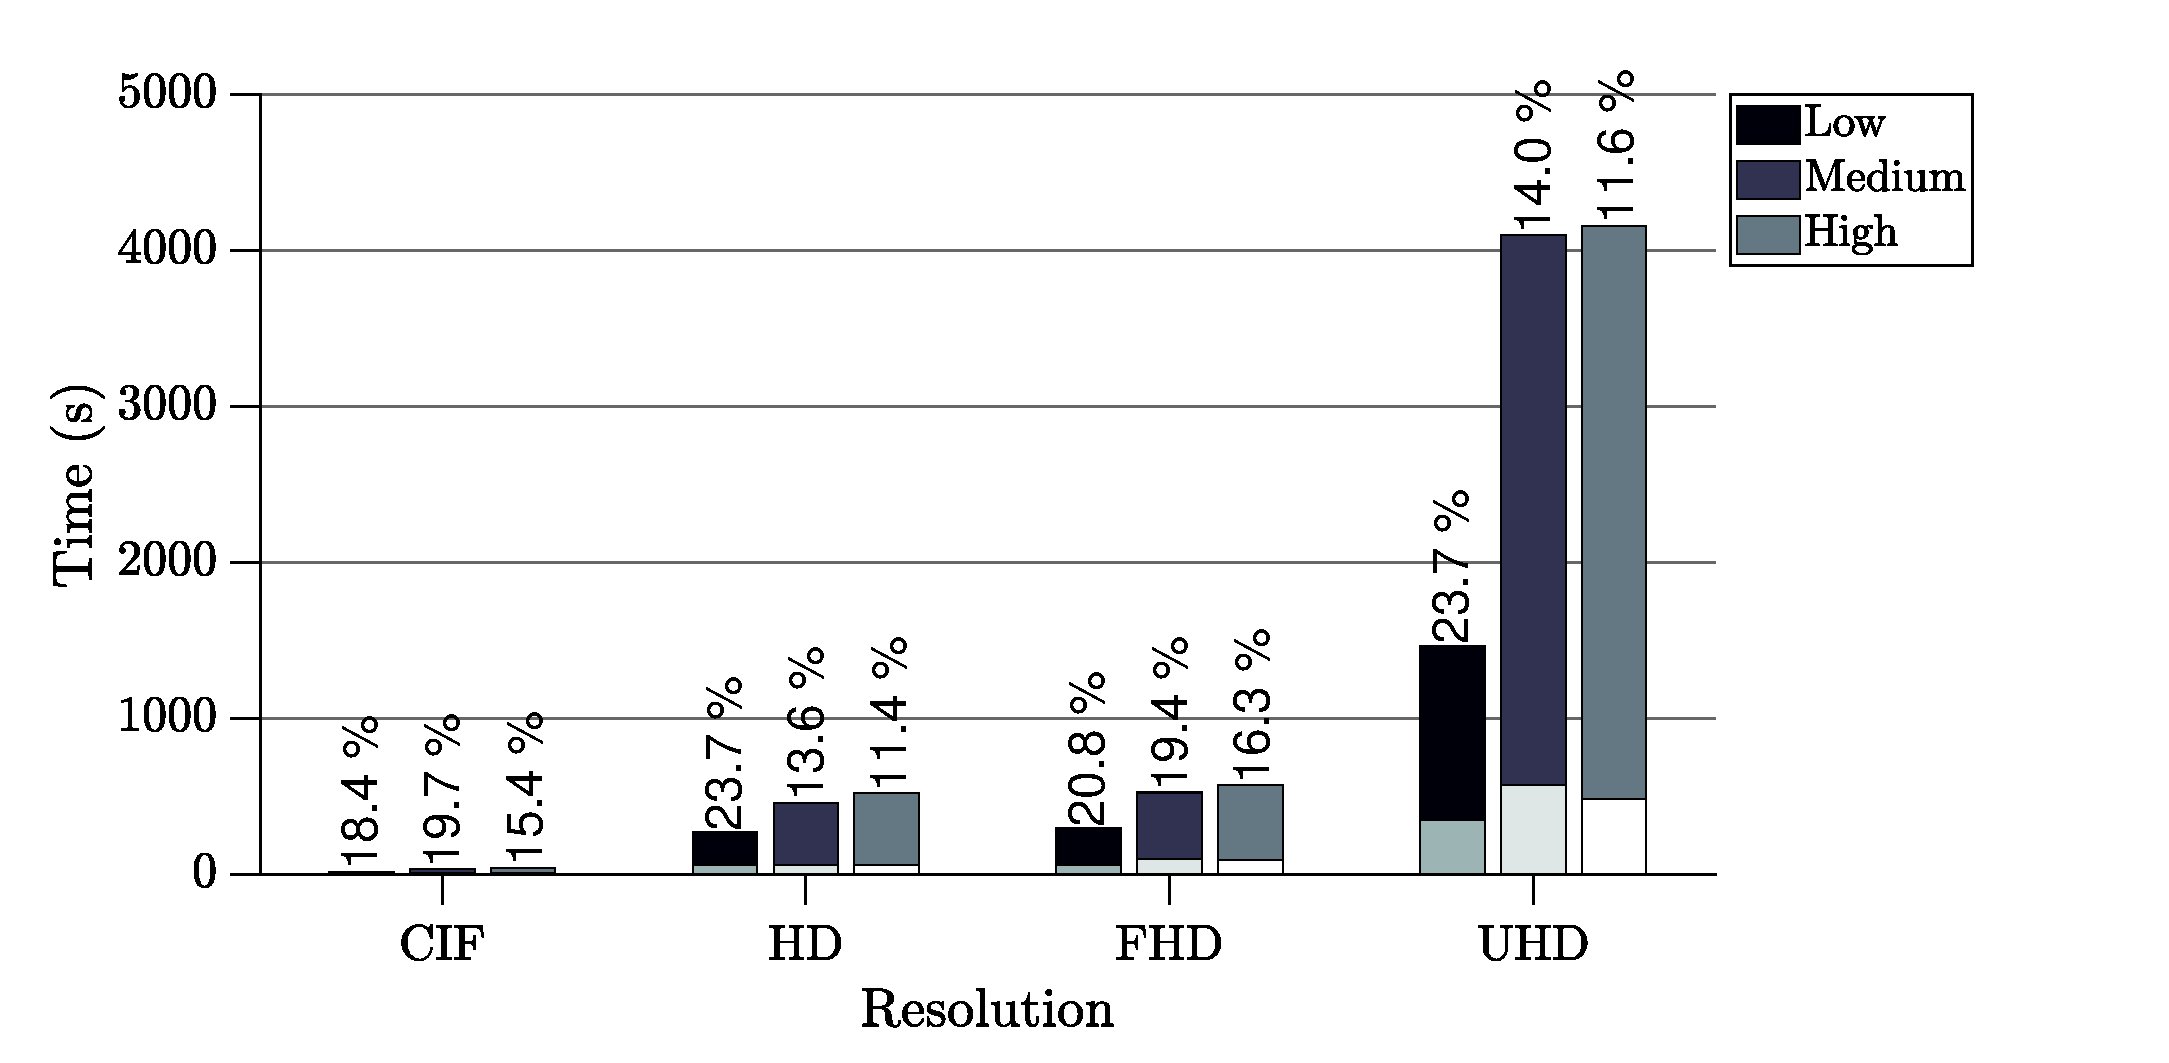
\includegraphics[width=\textwidth]{Sections/3Transforms/Images/TimingAnalysisAvg.eps}
    \caption[Average encoding and transform time per resolution, on different quality objectives]{Average encoding and transform time per resolution, on different quality objectives (dark colours represent total encoding time, while lighter are the respective time spent on transform stage)}
    \label{fig:timeavg}
\end{figure}

In this figure, each tall bar corresponds to the average time spent per encode, in each of the resolutions, varying the desired quality objective. The corresponding smaller bar represents the percentage of time spent during transformation, also expressed numerically by the number on top of each bar.

As anticipated, the desired quality of each encode plays an important role in the necessary total time, majorly considering the \emph{Low} to \emph{Medium} quality objectives, since the latter, in average, spends \emph{double} the time of the former. However, once considered the \emph{High} quality set, the encoder takes $14 \%$ more time to encode the same sequence on a \emph{Medium} quality objective.

Although these results represent an interesting analysis from a performance standpoint, for the focus of this work, the most interesting analysis comes from the percentage of time spent during the \emph{Transform} stage. As expected, this time stays roughly the same, independently of the quality objective. However its impact to the total encoding time decreases as the quality increases. 

This aspect leads to conclude that there is a necessity to develop fast and efficient architectures for the \emph{Transform} block, since it corresponds to a relevant percentage of the total encode time, regardless of the quality. And although lower quality encodes benefit more of such improvements when comparing to higher qualities, both cases would gain, since such architecture could be used on a high variety of encoders.

%%%%%%%%%%%%%%%%%%%
\subsubsection{Configuration Set Analysis}

This analysis is divided in different segments, dedicated to each of the transform options analyzed. Some of which, although not entirely relevant to the aim of this work, may prove useful for the implementation of different architectures.

On the distribution of used kernels verified in figure \ref{fig:kernelavg}, the most relevant aspect is the clear dominance of the \emph{DCT} among the others. However, as quality increases, the distribution starts to spread out.

\begin{figure}[!htpb]
    \centering
    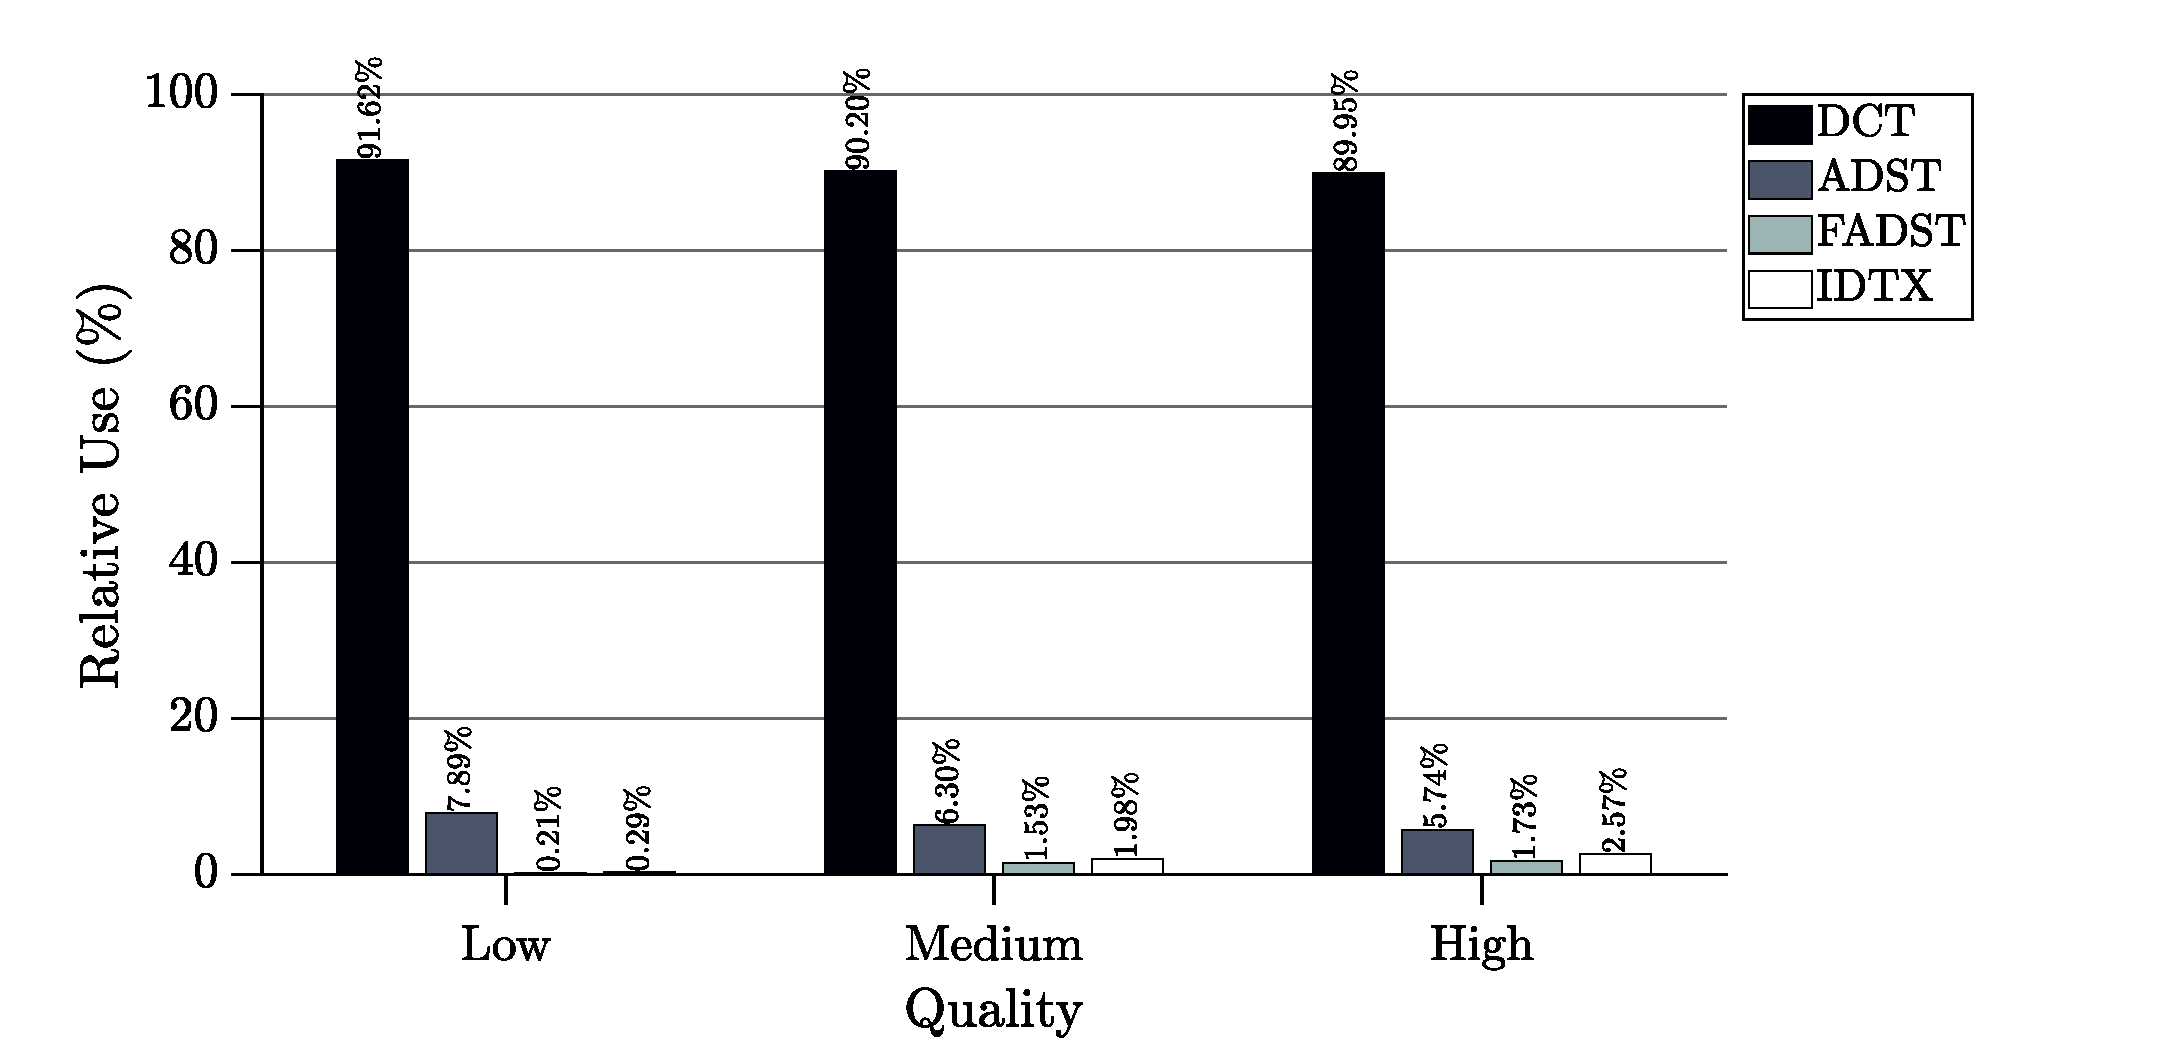
\includegraphics[width=\textwidth]{Sections/3Transforms/Images/kernelAvg.eps}
    \caption{Average distribution of used kernels, for all resolutions, according to the quality threshold}
    \label{fig:kernelavg}
\end{figure}

A contrary behavior is verified on the transform vector size. As seen in figure \ref{fig:sizeavg}, as quality increases, the smaller vector sizes (namely the $4$ length vector), get used more frequently. This is easily understandable, as smaller blocks present lower losses during the \emph{Quantization} stage. 

\begin{figure}[!htpb]
    \centering
    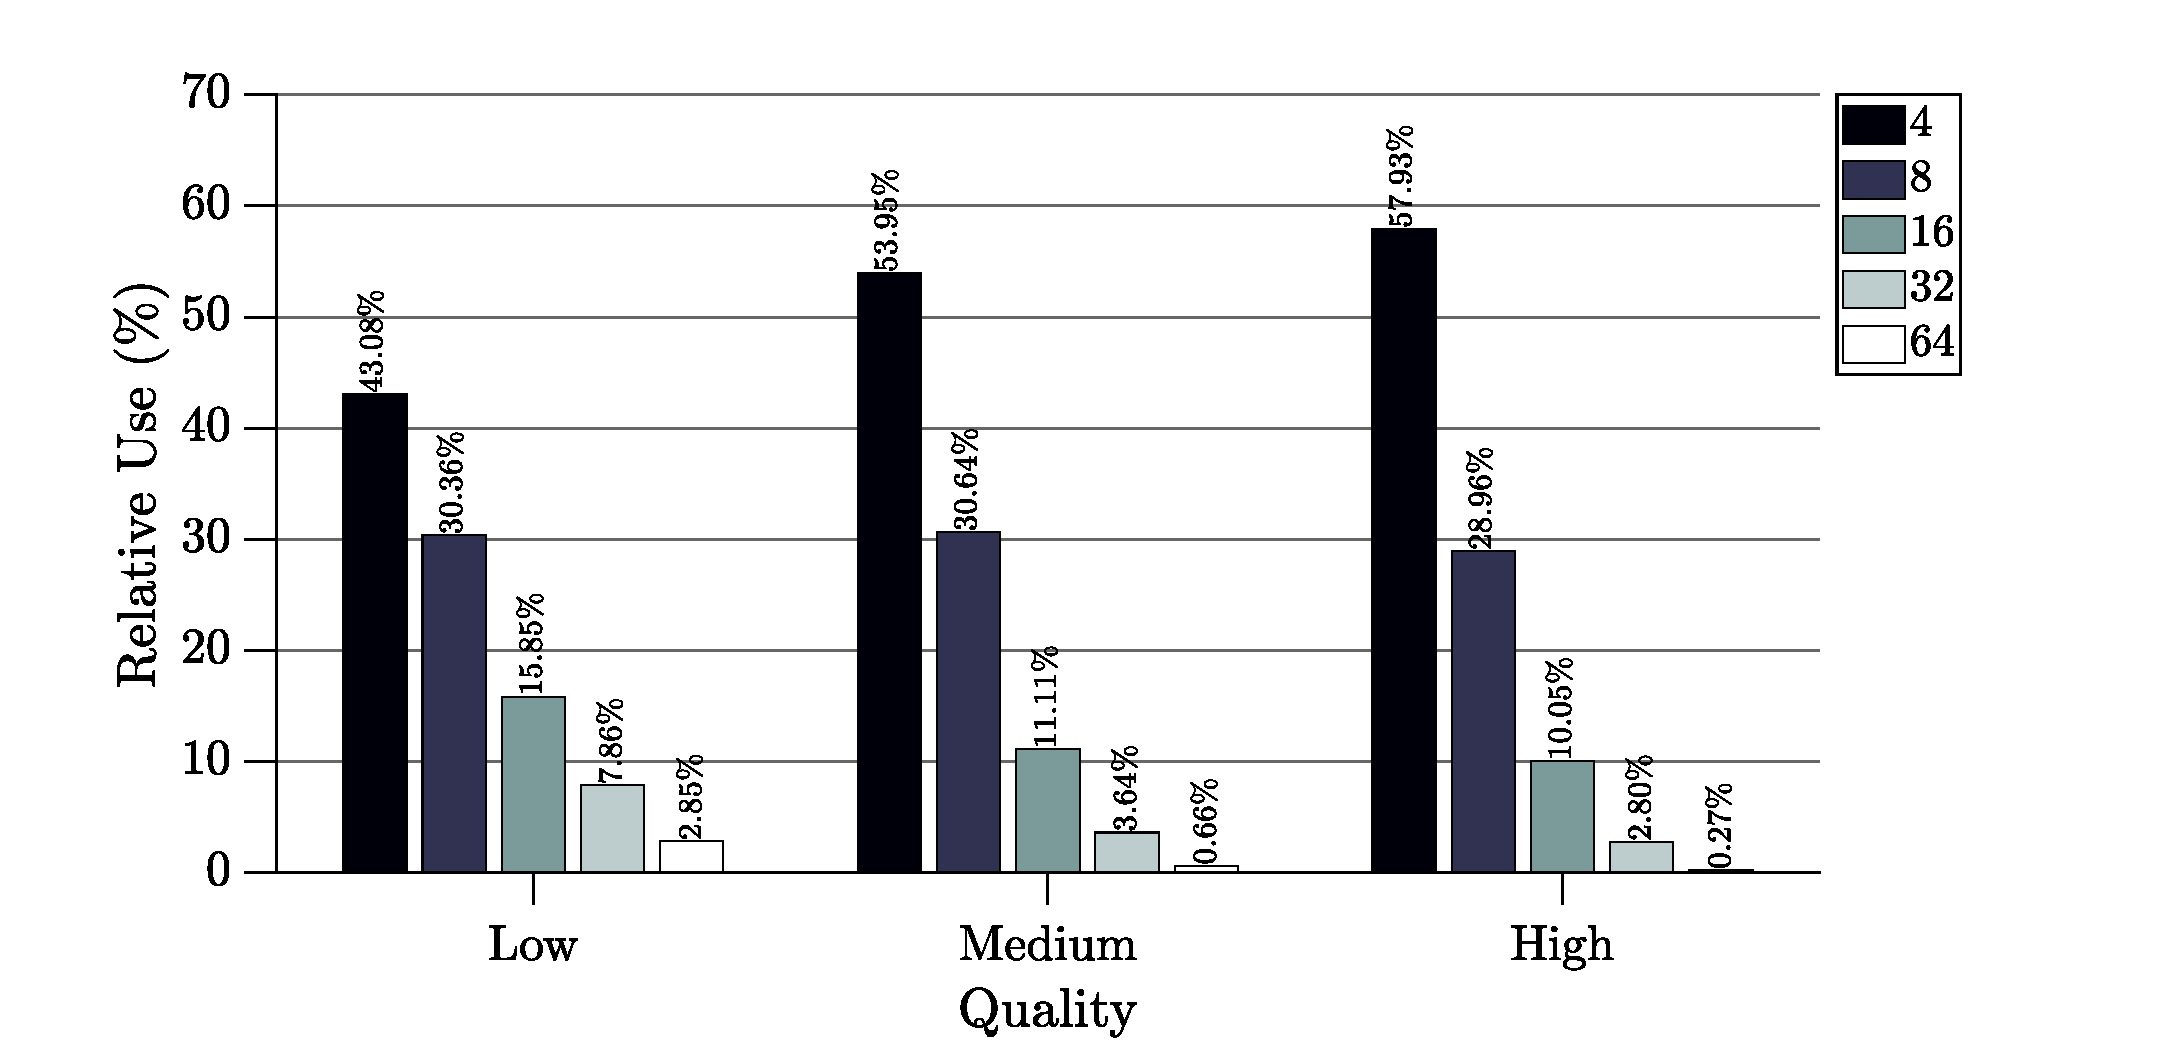
\includegraphics[width=\textwidth]{Sections/3Transforms/Images/vectSizAvg.eps}
    \caption{Average distribution of vector sizes, for all resolutions, according to the quality threshold}
    \label{fig:sizeavg}
\end{figure}

Although \emph{AV1} supports asymmetric transform blocks, in figure \ref{fig:squareavg} it's possible to verify that the encoder, in most of the block transformations, doesn't take advantage of such, using square blocks, as well as the same kernel for both directions. This behavior remains similar throughout the different resolutions.

\begin{figure}[!htpb]
    \centering
    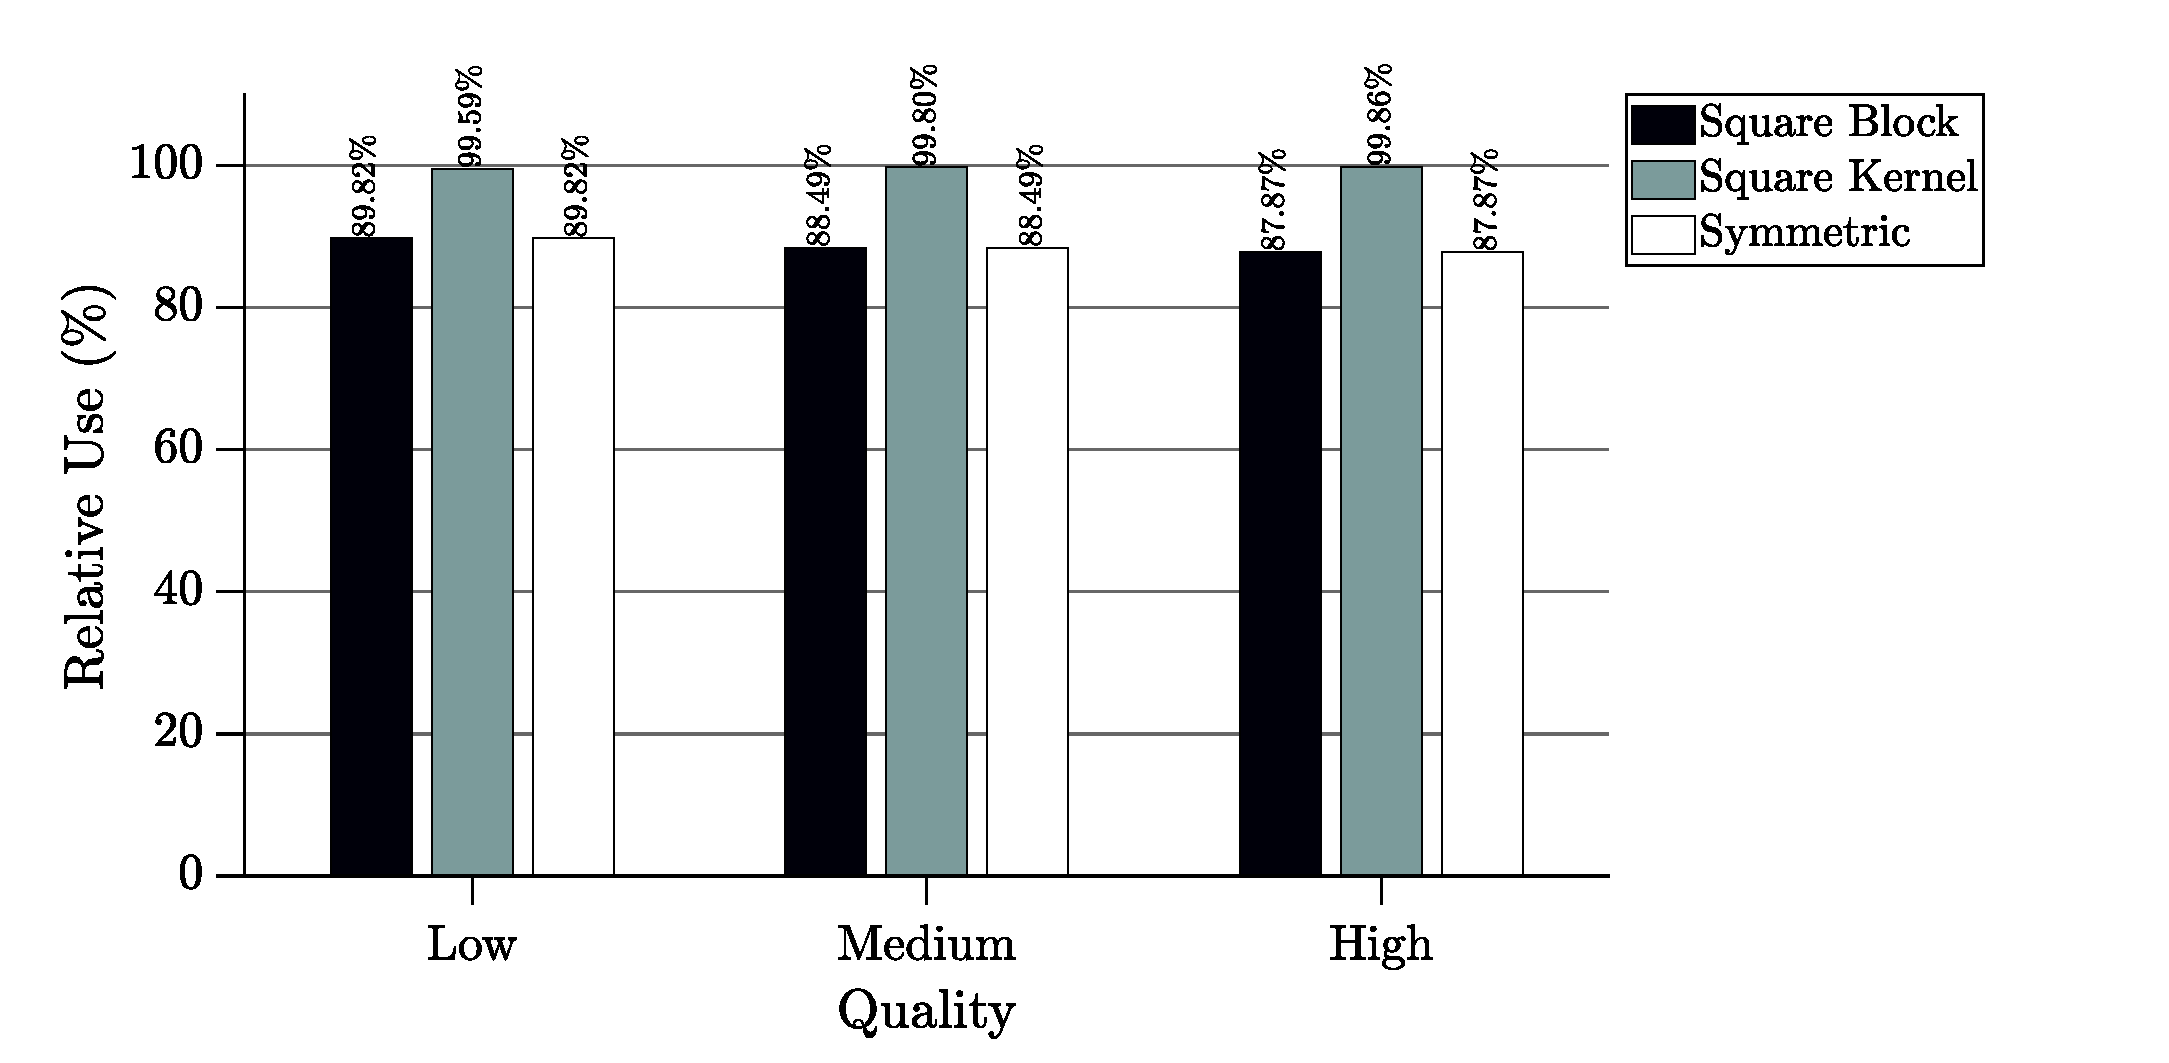
\includegraphics[width=\textwidth]{Sections/3Transforms/Images/squareAvg.eps}
    \caption{Use of square blocks, same kernel for rows and columns, and symmetric kernels, according to the quality threshold}
    \label{fig:squareavg}
\end{figure}

This aspect may prove a starting point for improvement of the transform stage, since, as mentioned previously, symmetric transforms may be implemented with \emph{\gls{mm}}. Therefore, using fast \emph{MM} architectures for symmetric blocks, and complementing with the algorithm implemented in \emph{libaom} for asymmetric blocks, the transform time may decrease.

The final analyzed transform option is the number of bits used in the cosine representation. In figure \ref{fig:cosbitavg}, the distribution is represented for the different quality objectives. 

\begin{figure}[!htpb]
    \centering
    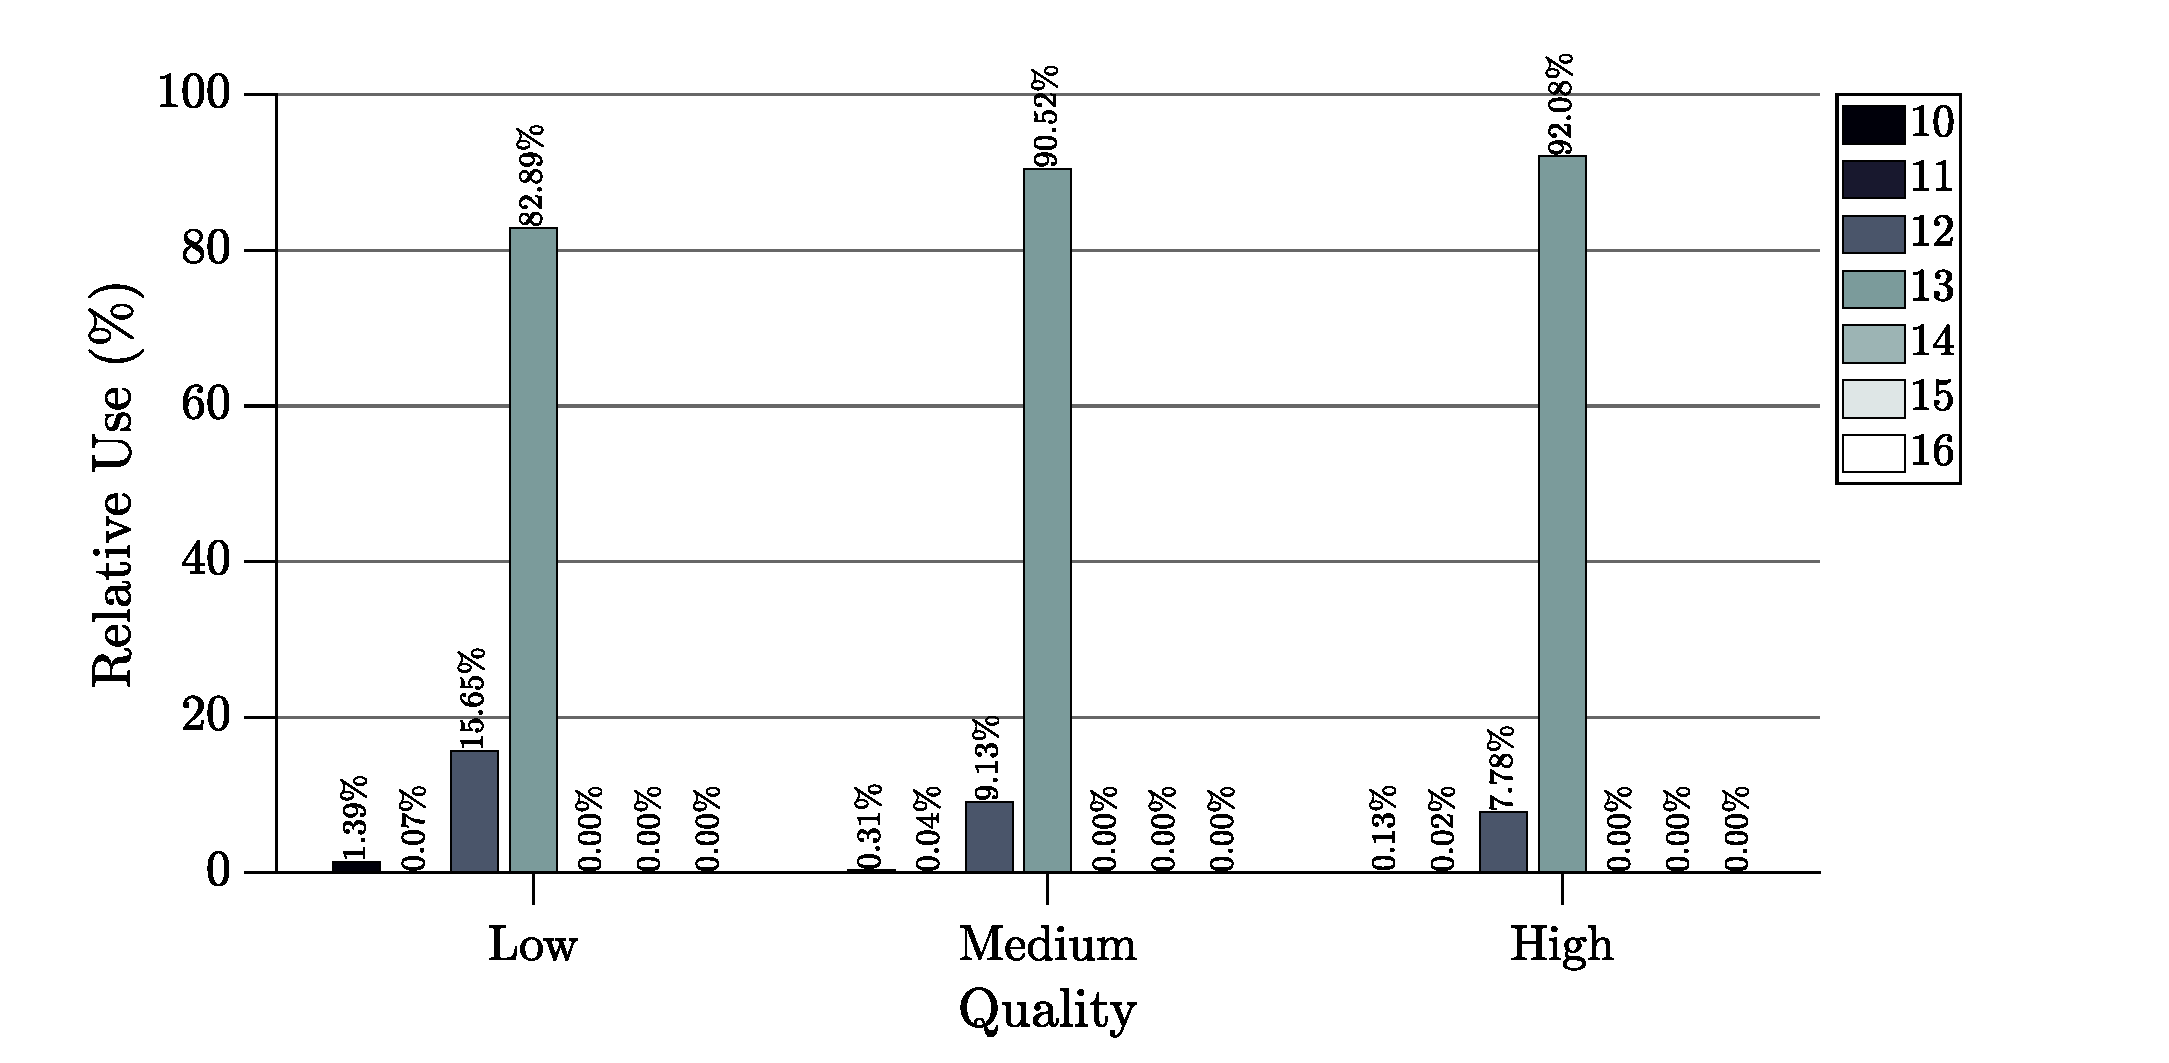
\includegraphics[width=\textwidth]{Sections/3Transforms/Images/cosBitAvg.eps}
    \caption{Different number of bits used on the cosine approximations, throughout different quality sets}
    \label{fig:cosbitavg}
\end{figure}

Various conclusions can be derived from this data.
Firstly, as expected, as quality increases, so does the number of bits for cosine representation, as seen by the increase of the percentage on the $13$ bit representation.

However, most representations hardly get used, since most of the transformations use $13$, $12$, $10$ and, very few times, $11$ bits, without using any of the higher representations (on the performed tests). 

Analyzing this information, it may be thought that the number of bits used in the cosine contributes for the overall quality of the compressed sequence. In the following section, this aspect is tested.

%%%%%%%%%%%%%%%%%%%
\subsubsection{Quality Analysis}

In this test, besides evaluating the obtained quality for each tested \texttt{cq-level}, the impact of the cosine bits representation also was evaluated. 

To evaluate the impact of the number of bits used in the cosine approximations, \emph{aomenc} was modified to force either 10 or 16 bits throughout the encoding operation, for both forward ($T$) and inverse transformations ($T^{-1}$). \emph{Aomdec} (reference decoder), since it acts according to the specified \emph{Bitstream Decoding Format} \cite{AV1BitstreamDecoding}, it may not be modified. Nonetheless, it uses $12$ bit representation, regardless of the choices made in the decoder.

From the gathered reconstructed sequences, $\hat{g}$, the \gls{psnr} of each one was calculated, according to equation \ref{eq:psnr}.

\begin{equation} \label{eq:psnr}
    PSNR = 10\;log_{10}\left(\frac{255^2}{E_{ms}}\right)
\end{equation}

$E_{ms}$ corresponds to the \emph{Mean Squared Error} of the reconstructed video. Considering a single $M \times N$ monochrome frame, this error is given by equation \ref{eq:emsf}.

\begin{equation} \label{eq:emsf}
    E_{ms} = \frac{1}{MN}\sum^{M-1}_{x=0} \sum^{N-1}_{y=0} \left(g_{x,y} - \hat{g}_{x,y}\right)^2
\end{equation}
However, since the test revolves around a sequence of $K$ reconstructed frames, with three chroma channels per bit, $c$, $E_{ms}$ becomes

\begin{equation} \label{eq:emss}
    E_{ms} = \frac{1}{3KMN}\sum^{K-1}_{k=0} \sum^{M-1}_{x=0} \sum^{N-1}_{y=0} \sum_{c=0}^{3-1} \left(g_{k,x,y,c} - \hat{g}_{k,x,y,c}\right)^2
\end{equation}

The workflow of the performed test is represented in figure \ref{fig:compcosbit}.

\begin{figure}[!htbp]
    \centering
    \begin{tikzpicture}[%
    >=triangle 60,              % Nice arrows; your taste may be different
    start chain=going right,    % General flow is top-to-bottom
    node distance=2cm,          % Global setup of box spacing
    every join/.style={norm},   % Default linetype for connecting boxes
    scale=0.75, every node/.style={transform shape},
    ]

\tikzset{
    base/.style={draw, on chain, on grid, align=center},
    proc/.style={base, rectangle, text width=2cm, fill=black!10, minimum height=1.5cm, minimum width=1.5cm,font={\bfseries}},    
    frame/.style={base, minimum height=1.5cm, minimum width=2cm, fill=blue!10, thick},
    sub/.style={base, circle, inner sep=0pt, radius=0.4cm, fill=black!10, minimum height=3.5ex, font={\bfseries}},
    spot/.style={circle, inner sep=0pt, radius=0.4cm, minimum height=2mm, draw},
    edge rectangle/.style={ to path={ rectangle (\tikztotarget)}},
    % coord node style is used for placing corners of connecting lines
    coord/.style={coordinate, on chain, on grid, node distance=6mm and 40mm},
    % Arrows 
    fforw/.style={->, thick},
    fback/.style={->, thick, red!75!black},
    aref/.style={<->, dashed, black!50},
    % -------------------------------------------------
    % Connector line styles for different parts of the diagram
    cascaded/.style = {%
    general shadow = {%
      shadow scale = 1,
      shadow xshift = -1ex,
      shadow yshift = 1ex,
      draw,
      thick,
      fill = blue!40},
    general shadow = {%
      shadow scale = 1,
      shadow xshift = -.5ex,
      shadow yshift = .5ex,
      draw,
      thick,
      fill =blue!40},
    fill = blue!40, 
    draw,
    thick,
    minimum width = 2cm,
    minimum height = 1.5cm,
    font={\itshape}},
    base
}

%% Reference
\node [cascaded] (inseq) {Sequência de\\Entrada};

\node [proc, right=3cm of inseq] (regenc) {Codificador\\Original};
    \draw[->] (inseq) -- (regenc);
\node [proc, above=of regenc] (bit10enc) {Codificador\\de 10 bits};
    \draw[->] (inseq)+(1.5cm,0) |- (bit10enc);
\node [proc, below=of regenc] (bit16enc) {Codificador\\de 16 bits};
    \draw[->] (inseq)+(1.5cm,0) |- (bit16enc);

\node [proc, right=3cm of regenc] (dec) {Desc.\\Original};
    \draw[->] (regenc) -- (dec);
    \draw[->] (bit10enc) --++(1.5cm,0) |- (dec.160);
    \draw[->] (bit16enc) --++(1.5cm,0) |- (dec.200);

\node [cascaded, right=3.5cm of dec] (regrec) {Reconstruída\\Normal};
    \draw[->] (dec) -- ([xshift=-1.3mm]regrec.west);
\node [cascaded, above=of regrec] (10bitrec) {Reconstruída\\10 bits};
    \draw[->] (dec.20) --++(0.5cm,0) |- ([xshift=-1.3mm]10bitrec.west);
\node [cascaded, below=of regrec] (16bitrec) {Reconstruída\\16 bits};
    \draw[->] (dec.340) --++(0.5cm,0) |- ([xshift=-1.3mm]16bitrec.west);

\node [proc, right=3cm of regrec, fill=black!15] (psnr) {Calcular \emph{PSNR}};
    \draw[->] (regrec) -- (psnr);
    \draw[->] (10bitrec) --++(1.5cm,0) |- (psnr.160);
    \draw[->] (16bitrec) --++(1.5cm,0) |- (psnr.200);

    \node[coord, below=3cm of inseq] (a) {};
    \node[coord, below=3cm of psnr] (aa) {};
    \draw[->] (inseq) -- (a) -- (aa) -- (psnr);
\end{tikzpicture}
    \caption{Description of the test for comparing impact of number of bits in cosine approximations}
    \label{fig:compcosbit}
\end{figure}

The average results from all resolutions, for each of the quality objectives is represented in figure \ref{fig:compcosbitavg}.

\begin{figure}[!htpb]
    \centering
    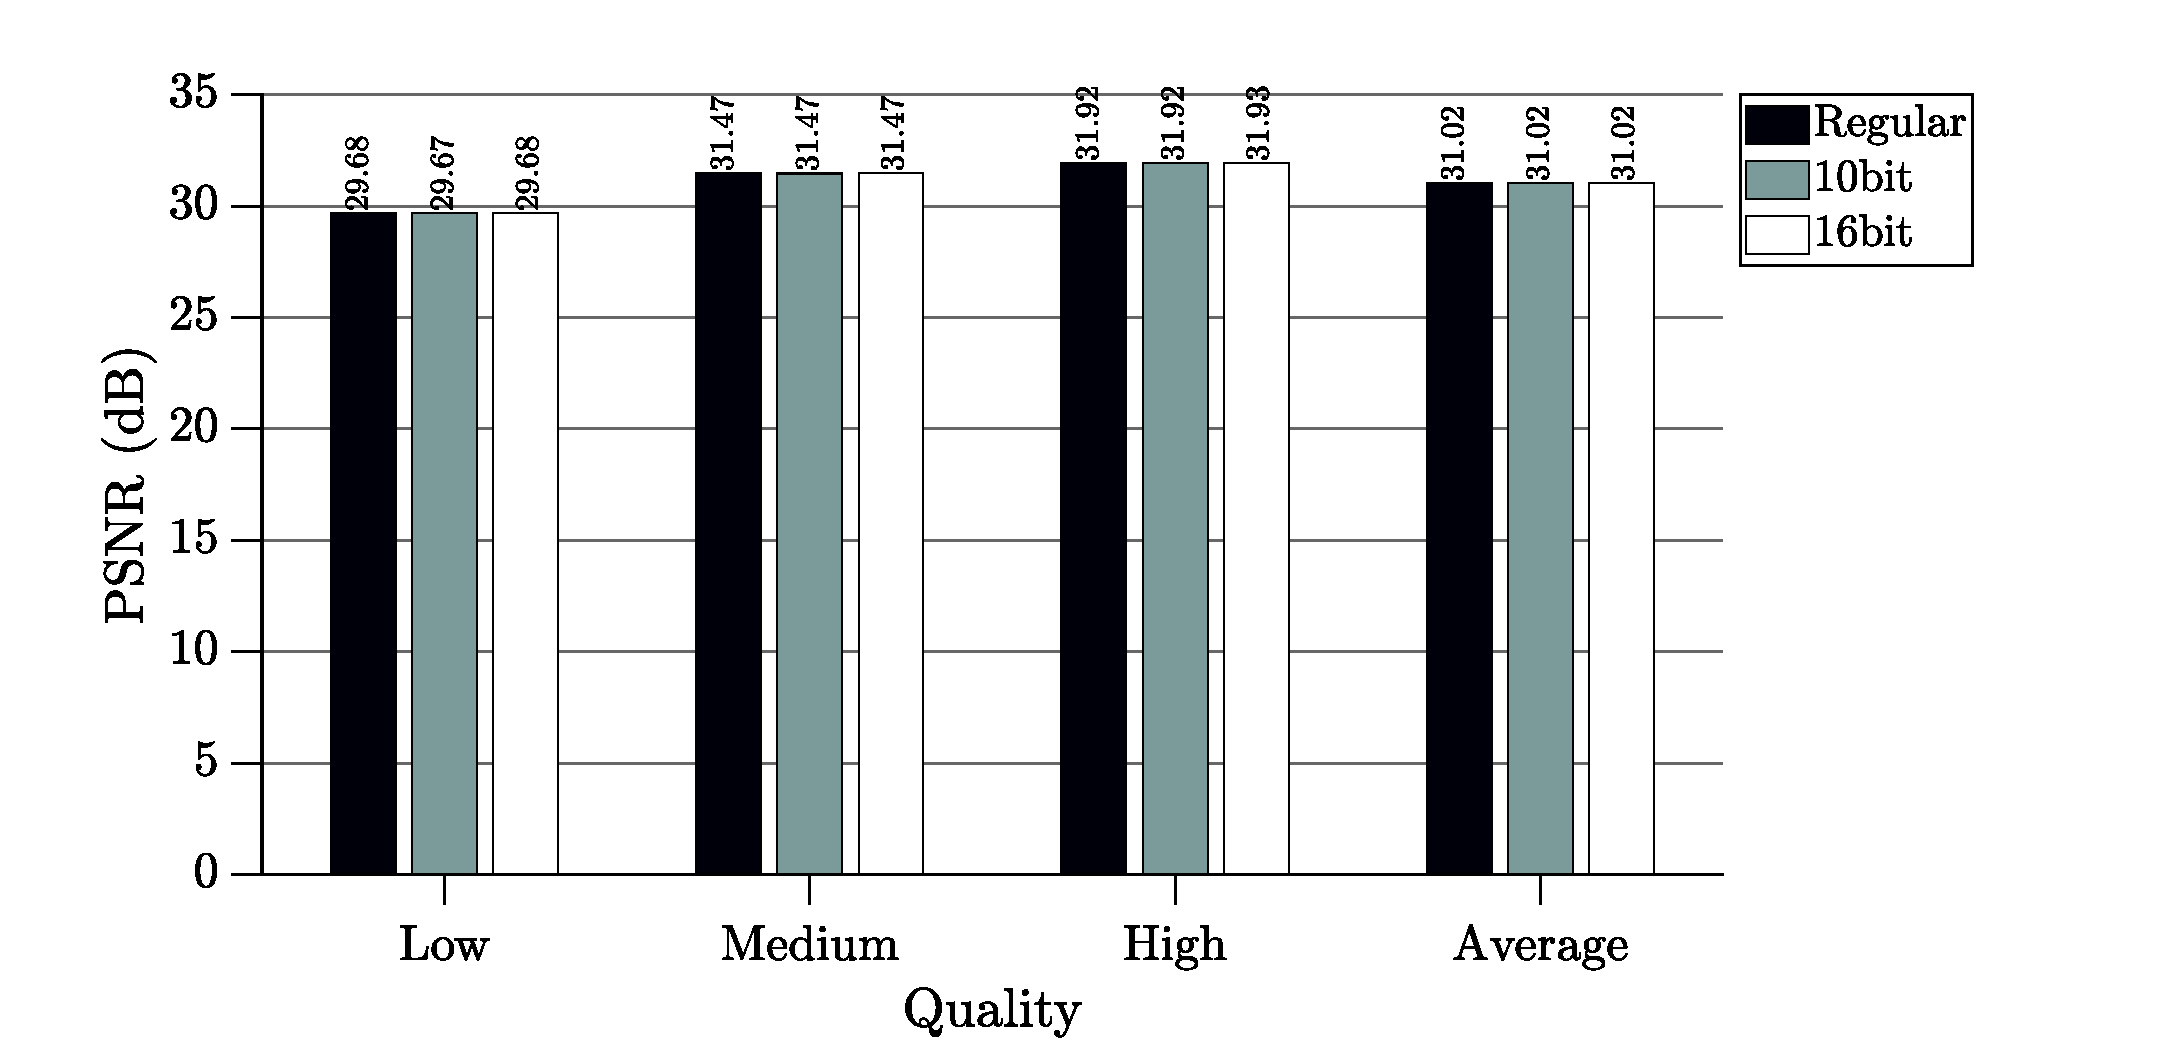
\includegraphics[width=\textwidth]{Sections/3Transforms/Images/compcosbitAvg.eps}
    \caption{Obtained quality for each of the quality objectives, and comparison with different cosine bits approximation}
    \label{fig:compcosbitavg}
\end{figure}

As expected, as \texttt{cq-level} increases, so does the obtained quality. Also, considering the encoding time differences verified in section \ref{sec:timinganal}, the smaller PSNR gap between \emph{Medium} and \emph{High} qualities was also expected. However, the difference between these two parameters depends on the encoded video, as shown in figure \ref{fig:qdiffs}, where the difference between \emph{Medium} and \emph{High} encodes is $2 dB$.

\begin{figure}[!htpb]
    \centering 
        \begin{subfigure}[c]{\textwidth}
            \centering
            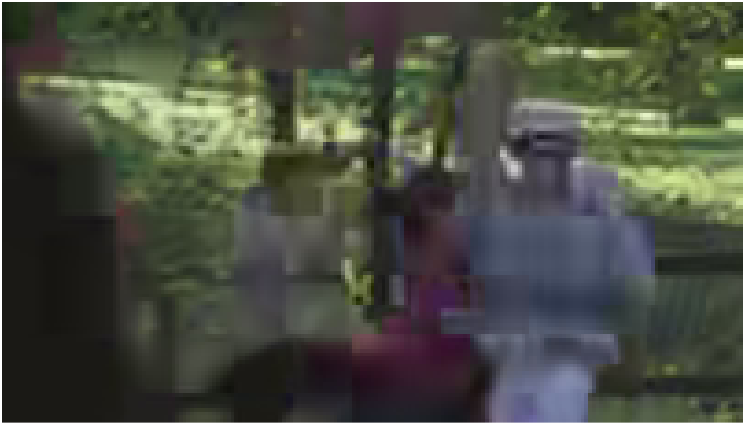
\includegraphics[height=0.25\textheight]{Sections/3Transforms/Images/lowParkDetail.png}
            \caption{\texttt{cq-level=60}}
            \label{subfig:lowq}
        \end{subfigure}
        \begin{subfigure}[c]{\textwidth}
            \centering
            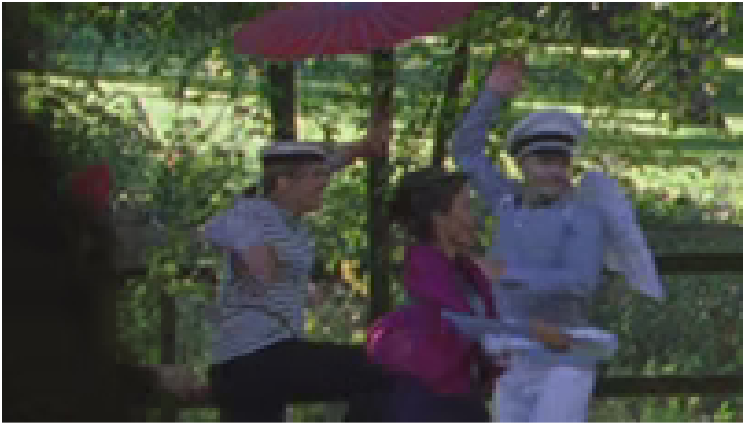
\includegraphics[height=0.25\textheight]{Sections/3Transforms/Images/medParkDetail.png}
            \caption{\texttt{cq-level=25}}
            \label{subfig:medq}
        \end{subfigure}
        \begin{subfigure}[c]{\textwidth}
            \centering
            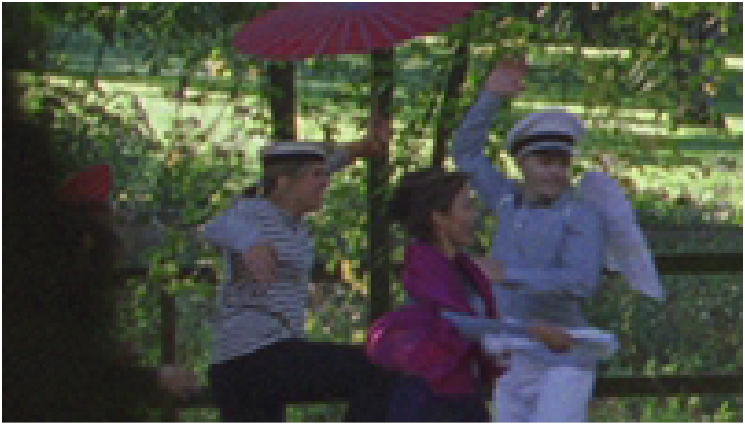
\includegraphics[height=0.25\textheight]{Sections/3Transforms/Images/highParkDetail.png}
            \caption{\texttt{cq-level=5}}
            \label{subfig:highq}
        \end{subfigure}
        \caption{Detail of \emph{Parkjoy} encodes, through different quality objectives}
    \label{fig:qdiffs}
\end{figure}

The differences between obtained PSNRs can be easily explained through analysis of the \emph{Quantization} stage in each quality objective. Looking at the distribution of the \emph{Quantizer/\Gls{qp}} 
\footnote{Parameter that indicates the \emph{quantization matrix} to use (higher values indicate more severe quantization).}
throughout the different \texttt{cq-level}'s (figure \ref{fig:quantavg}), it is possible to verify that this stage deeply adapts to the desired quality objective, increasing QP for lower qualities. 

\begin{figure}[!htpb]
    \centering
    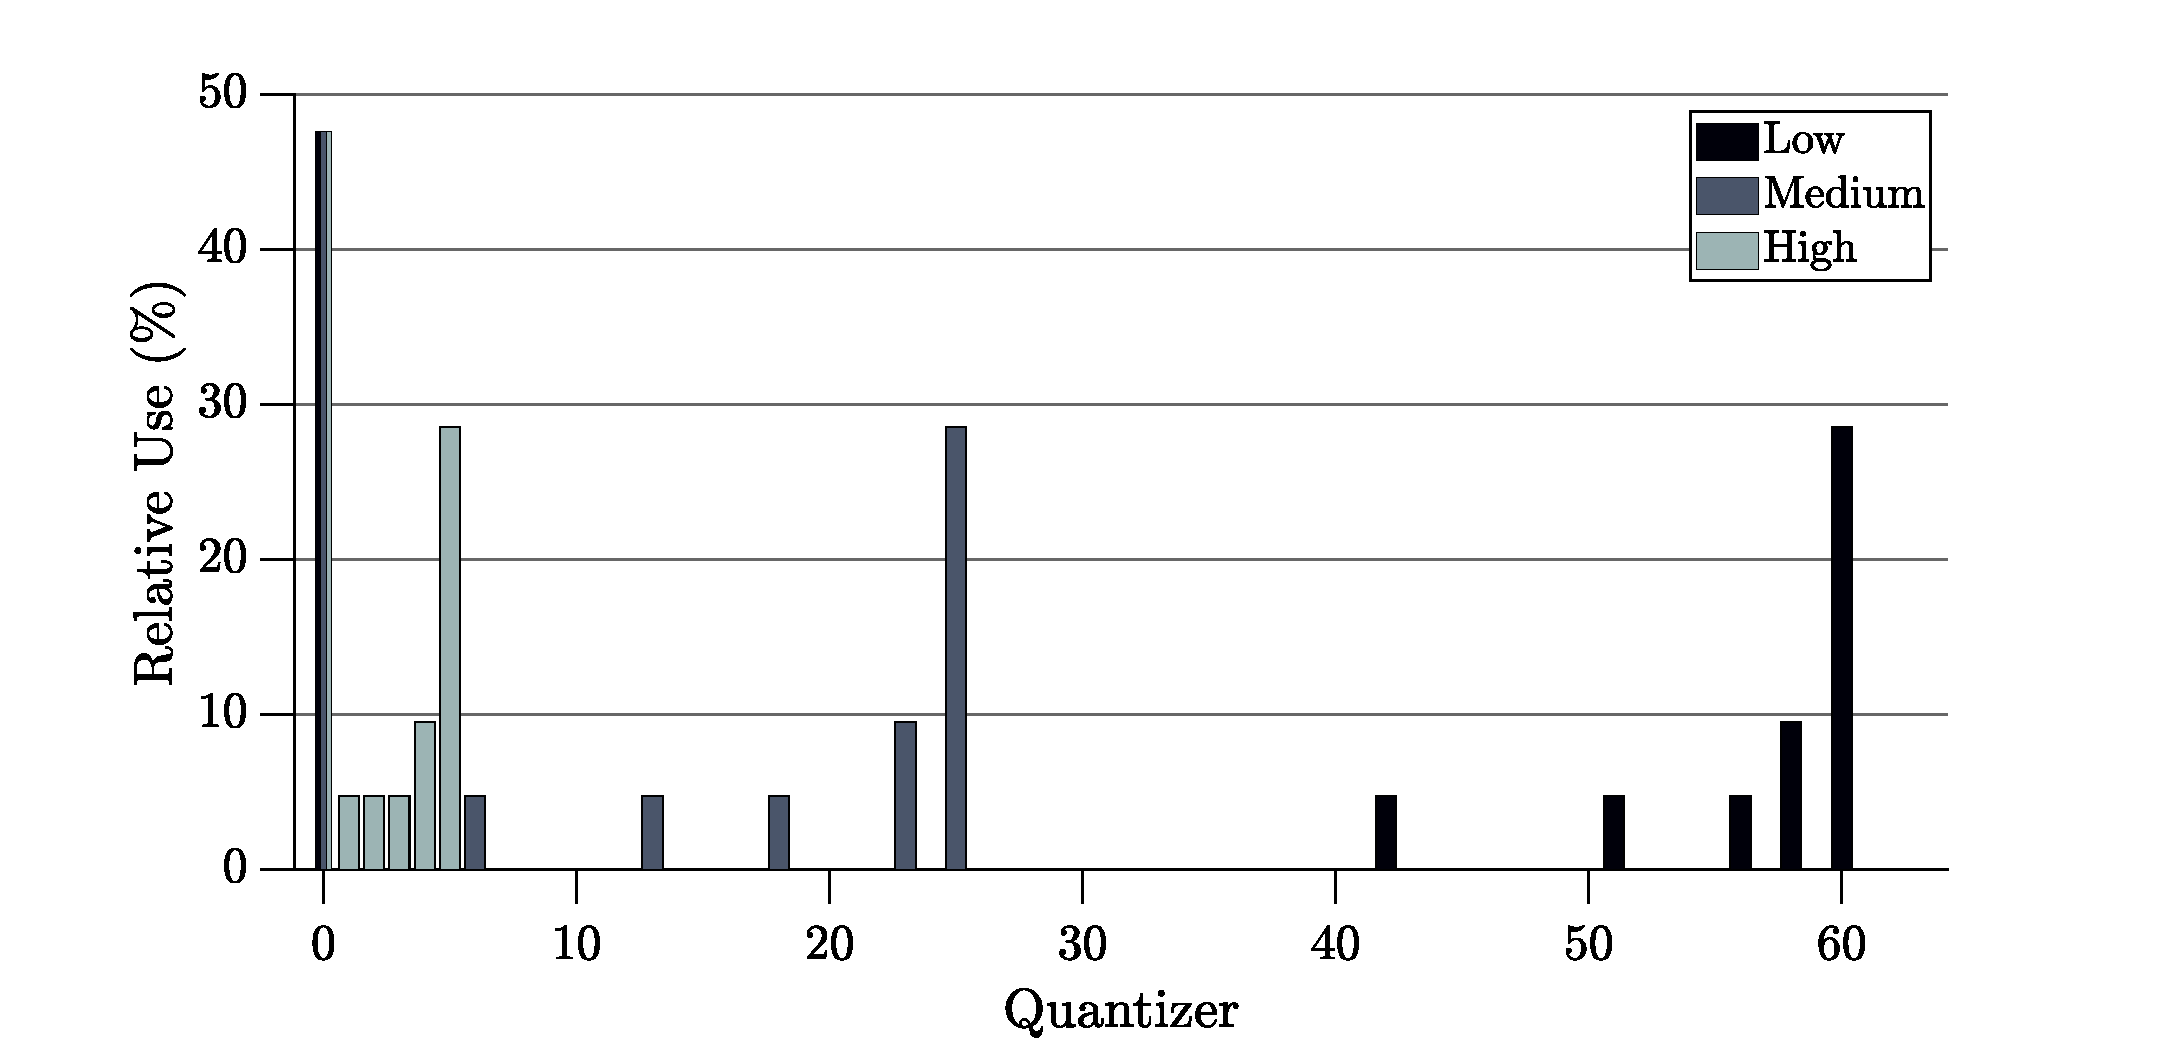
\includegraphics[width=\textwidth]{Sections/3Transforms/Images/quantizerAvg.eps}
    \caption{\emph{Quantizer} distribution on different quality objectives}
    \label{fig:quantavg}
\end{figure}

However, the differences in the used QP's don't justify the increased encoding time throughout the different quality objectives, since the \emph{Quantization} stage's complexity shouldn't vary depending on the desired quality, similarly to what happens on the \emph{Transform} stage. The time difference is mainly caused in the higher complexity blocks, the \emph{Inter} and \emph{Intra Prediction} stages, as the encoder adapts the processes in these blocks depending on the desired quality. For instance, there is no need for the encoder to make a exceptionally precise prediction, when most of the transform coefficients are discarded.

Considering now the obtained quality for each of the three different encodes (\emph{Regular}, \emph{10 bit} and \emph{16 bit}), it is possible to observe that the number of bits on cosine approximation doesn't contribute to the obtained quality, regardless of the desired objective, contrary to what was verified in figure \ref{fig:cosbitavg}. Accordingly, it would be safe to assume that the cosine approximations could be fixed on a certain number of bits, without major impact to the video quality.

This factor presents a major point for exploring faster \emph{Transform} block architectures. The architectures in figures \ref{fig:intDCT} and \ref{fig:intADST} are highly dependent on the \texttt{half\_btf} function (equation \ref{eq:half_btf}), which is adaptable to the number of bits used for cosine, in each block transformation. However, with the use of a fixed number of bits, this function could be simplified, since the multiplications and divisions performed in it could be implemented with a fixed number of shifts and additions.



\clearpage
\printbibliography[heading=subbibliography]
\addcontentsline{toc}{section}{References}